%%
%% Copyright 2007-2020 Elsevier Ltd
%%
%% 'Elsarticle Bundle'.
%% ---------------------------------------------


\documentclass[preprint,12pt,authoryear]{elsarticle}

\usepackage[latin1]{inputenc}
\usepackage[T1]{fontenc}
\usepackage{natbib}
\usepackage[nodisplayskipstretch]{setspace}
\usepackage{graphicx}
% Table convention: use tabular* with fill spacing, or tabularx, at textwidth.
\usepackage{tabularx}
\usepackage{threeparttable}
\usepackage{multirow}
		\usepackage{amsthm}
\usepackage{mathrsfs}
\usepackage{comment}
\usepackage{eurosym}
\usepackage{mathtools}
\usepackage{rotating}
\usepackage{amsmath,amssymb,amsthm,mathrsfs,amsfonts,dsfont}
\usepackage[tight]{subfigure}
\usepackage{color}
\usepackage{xcolor}
\usepackage{colortbl}
\usepackage{soul}
\newcommand{\mathcolorbox}[2]{\colorbox{#1}{$\displaystyle #2$}}
\usepackage{geometry}
\usepackage{times,mathpazo}
\usepackage[colorlinks,pdfborder={0 0 0},hypertexnames=false]{hyperref}
\usepackage{pict2e}
\usepackage{tikz}
\usepackage{lscape}
\usepackage{longtable}
\usepackage{subfigure}
\usepackage{tabu}
\usepackage{setspace}
\usepackage{threeparttable}
\usepackage{multirow}
\usepackage[capposition=top]{floatrow}
\usepackage{ragged2e}
\usepackage{pdfpages}
\usepackage{chngcntr}
\usepackage{float}
\usepackage{footmisc}
\usepackage{array}
\usepackage{booktabs}

\usepackage[pagewise]{lineno}

\definecolor{citecol}{rgb}{0,0,1}
\definecolor{anchor}{rgb}{1,0,0}
\hypersetup{citecolor=citecol}
\hypersetup{anchorcolor=anchor}
\hypersetup{linkcolor=anchor}
\geometry{hmargin=2.2cm,vmargin=2.2cm}
\renewcommand{\baselinestretch}{1.1}
\renewcommand{\thesubfigure}{(\Alph{subfigure})}
\setlength{\subfigcapskip}{-2em}
\setlength{\emergencystretch}{2em}
% Permit substantial floats to share pages with text.
\renewcommand{\topfraction}{0.9}
\renewcommand{\bottomfraction}{0.8}
\renewcommand{\textfraction}{0.08}
\renewcommand{\floatpagefraction}{0.75}
\setcounter{topnumber}{3}
\setcounter{bottomnumber}{2}
\setcounter{totalnumber}{4}
\setlength{\textfloatsep}{12pt plus 2pt minus 2pt}
\setlength{\intextsep}{12pt plus 2pt minus 2pt}
\setlength{\floatsep}{12pt plus 2pt minus 2pt}
\widowpenalty = 10000
\clubpenalty = 10000

\renewcommand\thefootnote{\textcolor{red}{\arabic{footnote}}}

\newcommand{\E}{\text{\textsf{E}}}
\newcommand{\rlo}{\rule[-0.20in]{0.0in}{0.1in}}
\newcommand{\rlobis}{\rule[-0.10in]{0.0in}{0.1in}}
\newcommand{\rhi}{\rule{0.0in}{0.30in}}
\newtheorem{proposition}{Proposition}
\newenvironment{proofcms}[1][Proof]{\noindent\textbf{#1.} }{\ \rule{0.5em}{0.5em}}

\newcommand*{\footnotemarkcolor}{black}
\makeatletter
\renewcommand*{\@makefnmark}{\hbox{\@textsuperscript{%
  \color{\footnotemarkcolor}\normalfont\@thefnmark}}}
\makeatother
\newcommand{\bv}[1]{\mathbf{#1}}


\newtheorem{lem}{Lemma}
\newtheorem{cor}{Corollary}
\newtheorem{assum}{Assumption}
\newtheorem{defin}{Definition}

\usepackage{placeins}

%%%%%%%%%%%%%%%%%%%%%%%%%%%%%%%%%%%%%%%%%%%%%%%
\usepackage{multirow} % Required for multirows
\usepackage{lscape}
\usepackage{pdflscape}
%\usepackage{gensymb}
\usepackage{adjustbox}
%%%%%%%%%%%%%%%%%%%%%%%%%%%%%%%%%%%%%%%%%%%%%%%


%====================================
%====================================
%=== Type of Appendix ===============
\def\isSupplementary{0}
%====================================
%====================================
%====================================


%====================================
%====================================
%=== Type of Appendix ===============
\def\isAnonymous{0}
%====================================
%====================================
%====================================


\usepackage{mdframed}




% Keep each float's explanation in the same paragraph as its bold title.
\usepackage{caption}
\captionsetup{format=plain,labelfont=bf,textfont=normalfont,font=small,
  justification=raggedright,singlelinecheck=false,position=top,skip=8pt}
\newcommand{\floatcaption}[2]{%
  \caption[#1]{\textbf{#1}%
    \if\relax\detokenize{#2}\relax\else.\space{\normalfont\footnotesize #2}\fi}%
}


\begin{document}

\begin{frontmatter}


\title{Sovereign Risk Spillovers across Countries and Sectors\tnoteref{t1}}


\if\isAnonymous0

\author[insta]{Beno\^it Mojon}
\affiliation[insta]{organization={Bank for International Settlements},%Department and Organization
            city={Basel},
            postcode={CH-4002},
            country={Switzerland}}

\author[instb]{Xavier Ragot}
\affiliation[instb]{organization={Sciences Po, CNRS, OFCE},%Department and Organization
            city={Paris},
            postcode={75007},
            country={France}}

\author[instc]{Jean-Paul Renne}
\affiliation[instc]{organization={University of Lausanne},%Department and Organization
            addressline={CH-1015 Lausanne},
            country={Switzerland}}
\tnotetext[t1]{We are grateful to R{\'e}gis Breton, Bryan Hardy, Swapan-Kumar Pradhan and Goetz von Peter for useful comments and help. All errors are ours. The views expressed in this paper are those of the authors and do not necessarily reflect the views of the Bank for International Settlements.}

\fi


\begin{abstract}
We study how sovereign default spreads through financial links across countries and sectors. Using a network reconstructed from public end-2024 data for Germany, France, Italy and Spain, we quantify how costly bank defaults can make repayment shortfalls reinforce one another. The same sovereign shock can then lead to different banking outcomes. We measure the resulting differences in creditor losses and compare guarantees with central-bank bond purchases. A credible repayment guarantee can eliminate the worse outcomes without paying out in equilibrium. Building on this established mechanism, we determine the minimum financial backing required by our guarantee rule: EUR~60.6 billion in the calibration. A backstop covering part of bank default losses also eliminates multiple equilibria, but requires payments. Purchases of sovereign bonds can also eliminate adverse banking outcomes, while transferring sovereign risk to the Eurosystem.
\end{abstract}


\begin{keyword}
%% keywords here, in the form: keyword \sep keyword
Sovereign risk \sep Financial networks \sep Bank default \sep Contingent public support
%% JEL codes here, in the form: \JEL code \sep code
\JEL G01 \sep G21 \sep H63
\end{keyword}

\end{frontmatter}

% To have lines numbers:
%\linenumbers


% \newpage


% \begin{center}
% \begin{large}
% Conflict-of-interest disclosure statement
% \end{large}
% \end{center}

% \vspace{2cm}

% Jean-Paul Renne
% \vspace{.5cm}

% I have nothing to disclose.

% \vspace{2cm}

% Kevin Pallara
% \vspace{.5cm}

% I have nothing to disclose.


% \newpage

\setstretch{1.5}


\section{Introduction}

Sovereign distress can weaken banks through their government bond holdings and spread through domestic and cross-border financial claims. Initial losses are only part of the problem: one bank's repayment shortfall can cause others to repay less, allowing both high- and low-repayment outcomes after the same sovereign shock. We study this feedback and compare two ways to contain it: guarantees covering shortfalls in interbank repayments, and central-bank purchases reducing banks' sovereign exposure before the shock.

Our empirical contribution is a reconstruction of the financial exposure network for Germany, France, Italy and Spain from public end-2024 data. It covers banks, nonbank financial institutions, households, firms, governments and the Eurosystem. We classify financial claims by the countries of the creditor and debtor, and combine data sources to match published totals for each financial instrument. Where bilateral exposures are unavailable, we allocate the published totals across counterparties using stated assumptions. The numerical results therefore depend on these allocations and the assumed crisis losses. Using the same network, we compare direct sovereign losses, the additional losses caused by repayment shortfalls and the effects of alternative interventions.

We use the network in a model that determines banks' debt payments jointly for each sovereign-default scenario. A costly bank default destroys a fixed fraction of the bank's remaining asset value, representing losses from disrupted operations and the difficulty of selling assets during distress. These default costs are additional to the losses on sovereign bonds and claims on other banks that bring the bank into distress. Interbank claims transmit losses even without default costs, as in \citet{EisenbergNoe2001}. Without these costs, our model has a unique banking equilibrium because every bank owes some of its debt to nonbank creditors, including depositors. With default costs, payments to creditors can fall abruptly when a bank enters distress. Banks can repay fully when their counterparties repay fully, yet default when their counterparties pay less. The additional asset destruction then deepens repayment shortfalls, allowing defaults to sustain one another. Each of the four sovereigns can default or repay as promised, giving sixteen sovereign scenarios. Eight admit multiple banking equilibria in the baseline calibration.

Our guarantee analysis determines the financial backing needed to make the highest-repayment equilibrium unique. In this equilibrium, every bank repays at least as much as in any other equilibrium after the same sovereign shock. Some banks may still default in this outcome. The repayment floor promises interbank creditors at least what this outcome would pay them. The idea that credible guarantees can eliminate self-fulfilling repayment shortfalls without requiring payments in equilibrium is established \citep{DiamondDybvig1983,JacksonPernoud2021}. Proposition~\ref{prop:greatest-floor} shows that a fully honoured repayment floor makes the highest-repayment equilibrium unique, with zero guarantee payments in equilibrium. When total guarantee claims exceed the facility's capacity, every claimant receives the same fraction of its claim. Creditors anticipate this proportional rationing. Proposition~\ref{prop:critical-floor-budget} identifies the critical capacity above which the highest-repayment equilibrium is unique and establishes whether that capacity itself suffices. In the calibration, EUR~60.6 billion is the smallest facility capacity that ensures a unique equilibrium in every sovereign scenario. This is 52\% below the largest bill for compensating interbank creditors after an adverse outcome has occurred.

The recovery backstop reimburses interbank creditors for a specified fraction of the repayment capacity destroyed by bank default costs, with total receipts capped at the amount owed. Payments are calculated from the defaulting bank's remaining assets and the fraction of asset value lost in distress. By reducing the losses passed to creditor banks, the backstop weakens the feedback that sustains further defaults and makes the equilibrium unique in the calibration. The two guarantees therefore cover different losses: the repayment floor covers shortfalls below the original highest-repayment outcome, while the backstop compensates for asset destruction whenever a debtor bank defaults. Defaults that persist in equilibrium consequently require backstop payments, even though the repayment floor would pay nothing at its target outcome.

The bond-purchase experiment examines how quantitative easing (QE) can reduce repayment feedback. Exchanging banks' sovereign bonds for safe Eurosystem reserves changes which banking equilibria can arise, even with asset prices and lending held fixed. The composition of purchases matters. Buying half of banks' French sovereign holdings makes the banking equilibrium unique, while leaving unchanged the defaults that occur even under full interbank repayment. Buying three quarters of their Italian and Spanish holdings makes full bank repayment an equilibrium in every sovereign state, but outcomes with mutually reinforcing bank defaults remain possible. Thus reducing direct sovereign losses need not eliminate self-sustaining repayment shortfalls. Purchases transfer sovereign risk to the Eurosystem, whereas the repayment floor supports interbank repayments through a promise to cover shortfalls.

The analysis builds on \citet{RogersVeraart2013}, who study interbank repayment with default costs and bank rescue. \citet{JacksonPernoud2024} study the minimum capital injections needed to restore systemic solvency, including interventions that eliminate equilibria with defaults, and guarantees on network payments. Our contribution is to determine the financial backing required by the specified repayment-floor rule when creditors anticipate proportional rationing. Related work examines how defaults spread through financial claims \citep{ElliottGolubJackson2014} and the distinction between funds committed to a guarantee and payments actually made \citep{RochUhlig2018}.

We also contribute to the literature on the links between sovereign and bank distress. \citet{GennaioliMartinRossi2014}, \citet{AcharyaDrechslerSchnabl2014} and \citet{Bocola2016} study how sovereign distress, bank funding and lending interact. At the macroeconomic level, \citet{vonPeter2009} examines feedback between asset prices, borrower defaults and bank credit. Our analysis isolates how repayment shortfalls spread through a reconstructed cross-country network, holding financial exposures and the losses caused directly by the crisis fixed.

The purchase exercise complements the QE literature on bond yields and transmission channels \citep{GagnonEtAl2011,KrishnamurthyVissingJorgensen2011,AltavillaCarboniMotto2021}. \citet{AcharyaEisertEufingerHirsch2019} study how the European Central Bank's (ECB) announcement of Outright Monetary Transactions (OMT) raised sovereign-bond values, strengthened banks and affected lending. We examine how transferring sovereign exposure from banks to the Eurosystem changes repayment feedback and the banking equilibria that can arise. Holding asset prices and lending fixed allows us to identify how these purchases affect the spread of repayment shortfalls through financial claims.

Section~\ref{sec:model} presents the model and Section~\ref{sec:calibration} summarizes the calibration. Section~\ref{sec:multiple-equilibria} explains the banking outcomes. Sections~\ref{sec:ex-post-compensation} and~\ref{sec:interbank-recovery-backstop} study guarantees, and Section~\ref{sec:eurosystem-purchases} examines bond purchases. The appendices give implementation details, robustness results and the public-data construction.

\section{Model}\label{sec:model}

The model describes how a given sovereign shock propagates through financial claims. Exposures are in place at date 1. At date 2, sovereign repayments are specified by the scenario and banks settle their debts jointly. The analysis takes these exposures and repayment resources as given; it does not require a model of how firms and households chose their positions. An optional household-saving completion is provided in Appendix~\ref{app:household-completion}.

\subsection{Exposures and sovereign shocks}

There are $C$ countries, collected in $\mathcal C$. Country indices are $c$ or $g$; indices $i,j$ identify network nodes and are restricted to banks where indicated. Each country has households $H_c$, firms $F_c$, banks $B_c$, nonbank financial institutions (NBFIs) $N_c$ and a government $G_c$. Each bank node is a national block; claims within it represent lending among distinct institutions. The network also includes the Eurosystem $E$ and Other counterparties $R$. Write $\mathcal N$ for all nodes and $\mathcal B$, $\mathcal M$ and $\mathcal G$ for banks, NBFIs and governments. The Other counterparties node groups foreign and unclassified positions whose repayments are taken as given.

A claim $x_{ij}\geq0$ runs from creditor $i$ to debtor $j$: rows of the exposure matrix are creditors and columns are debtors. Bank debt $D_i>0$ denotes the liabilities sharing a common repayment rate. Obligations settled at fixed amounts outside this pool are called fixed settlements; they are deducted from both liabilities and repayment resources. The matrix covers selected instruments; its reconciliation with complete balance sheets supplies the remaining net resources. These accounting details are set out in Appendix~\ref{app:calibration-details}.

A sovereign state $s$ specifies default indicators $\delta_c^G(s)\in\{0,1\}$ for each country $c\in\mathcal C$. There are therefore $2^C$ possible sovereign states. Let $\overline r_c^G$ be government $c$'s contractual gross payment per unit of debt securities and $\underline r_c^G$ its payment following default. Its realized payment is
\[
 R_c^G(s)=\begin{cases}
 \overline r_c^G,&\delta_c^G(s)=0,\\
 \underline r_c^G,&\delta_c^G(s)=1,
 \end{cases}
 \qquad 0\leq\underline r_c^G<\overline r_c^G.
\]
These repayments are exogenous: banking outcomes do not change sovereign default or recovery. The scenario also specifies impairments on bank-held firm and household loans. Private borrowing and credit supply remain fixed during clearing.

Other counterparties and the Eurosystem repay at the safe gross rate, normalized to one. They bear losses on their assets without passing them back through their own debt payments. NBFIs also repay in full in the calibration.\footnote{The calibrated buffers imply full NBFI repayment even when their repayments are determined endogenously. Under national pooling and with other net resources fixed, these buffers cover all debt even if the selected claims on banks, other NBFIs and sovereigns pay nothing. Full repayment therefore holds in every equilibrium; Appendix~\ref{app:calibration-details} gives the bound.} Nonbank receipts are therefore fixed within each sovereign state in the reported exercises.

\subsection{Bank resources, distress and repayment}\label{sec:model_banks}

Normalize contractual bank repayment to one. For each bank block $i\in\mathcal B$, $R_i\in[0,1]$ is both the amount paid per unit borrowed and the creditor recovery rate; a claim of size $x_{ji}$ pays $x_{ji}R_i$. Collect these rates in the vector $\mathbf{R}=(R_j)_{j\in\mathcal B}\in\mathcal K$, where $\mathcal K=[0,1]^{|\mathcal B|}$.

Let $a_i(s)\geq0$ collect nonbank receipts net of fixed settlements and the scenario's losses. Bank $i$'s resources before its own default cost are
\[
 A_i(s,\mathbf{R})=a_i(s)+\sum_{j\in\mathcal B}x_{ij}R_j.
\]
We suppress the arguments $(s,\mathbf{R})$ when they are clear from context.

Let $E_i$ denote accounting equity in the reference balance sheet, whose repayment resources are $D_i+E_i$. Define the change in resources relative to this benchmark by
\[
 L_i=D_i+E_i-A_i,
 \qquad A_i-D_i=E_i-L_i.
\]
Thus $L_i>0$ measures the reduction in resources before the bank's own default cost; $L_i<0$ represents a gain relative to the benchmark. We refer to positive $L_i$ as pre-cost losses. These losses first reduce equity and need not entail losses for creditors. The quantity $E_i-L_i$ is remaining pre-cost equity when positive and an accounting shortfall when negative.

Loss headroom $0\leq H_i\leq E_i$ specifies how much of this reduction can occur before the distress threshold is breached. A breach occurs when $L_i>H_i$, equivalently $A_i<D_i+E_i-H_i$. Headroom sets the trigger; all accounting equity remains available to absorb losses. In particular, when $H_i<L_i<E_i$, the threshold is breached even though pre-cost equity remains positive.

A distress episode destroys the fraction $1-\lambda_i^B$ of the remaining estate, where $0<\lambda_i^B\leq1$. This wedge captures franchise disruption and difficult asset realization. It is a cost parameter, not a creditor recovery rate. Partial repayment requires both a headroom breach and a creditor shortfall after this cost:
\begin{equation}
 R_i=\begin{cases}
 \lambda_i^B A_i/D_i,&L_i>H_i\ \text{and}\ \lambda_i^B A_i<D_i,\\
 1,&\text{otherwise}.
 \end{cases}
 \label{eq:bank_repayment}
\end{equation}
Figure~\ref{fig:equity-headroom} illustrates three cases. Within headroom, the bank repays in full. After a breach, repayment remains full if pre-cost equity covers the hypothetical distress cost, $E_i-L_i\geq(1-\lambda_i^B)A_i$, equivalently $\lambda_i^B A_i\geq D_i$. Otherwise, the cost leaves insufficient resources to repay creditors in full. This can occur even with positive pre-cost equity. Figure~\ref{fig:bank-repayment-rule} summarizes the two tests. The rule is a reduced-form description of disorderly distress; a prudential breach is not an automatic legal default.

\begin{figure}[htbp]
\centering
\floatcaption{Headroom, equity and creditor losses: three balance sheets}{Illustrative balance sheets with the same debt, initial equity, headroom and cost parameter. The vertical arrow measures the resource threshold $D_i+E_i-H_i$ from the common zero baseline to the dashed line. Resources below this line breach headroom. Orange indicates the hypothetical distress cost; the solid line below it marks $\lambda_i^B A_i$. In (b), remaining equity covers this cost, so the model specifies full repayment. In (c), the cost exceeds remaining equity and creditors incur losses even though pre-cost equity is positive. The cost is applied only when both conditions in equation~\eqref{eq:bank_repayment} hold.}
\label{fig:equity-headroom}

\resizebox{0.98\textwidth}{!}{%
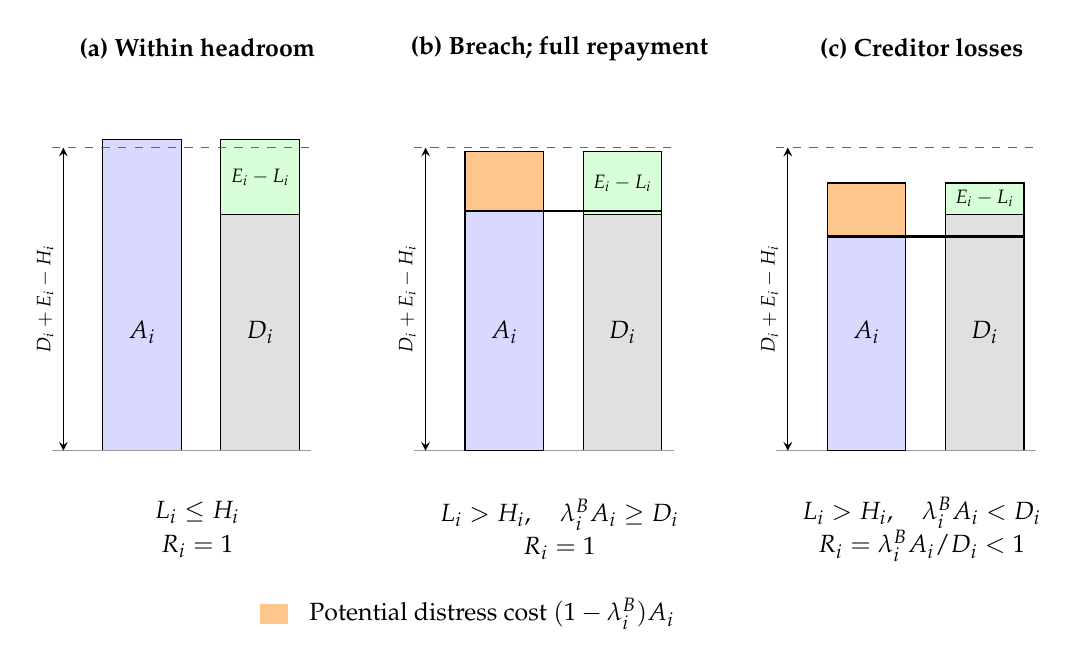
\begin{tikzpicture}[x=1cm,y=1cm,>=stealth,font=\small]
% Common illustrative values: D=3, E=1, H=.15, lambda=.8.
\foreach \shift/\height/\title in {0/3.95/{(a) Within headroom},4.6/3.8/{(b) Breach; full repayment},9.2/3.4/{(c) Creditor losses}} {
 \begin{scope}[xshift=\shift cm]
  \node[font=\small\bfseries,align=center] at (1.2,5.1) {\title};
  \fill[blue!15] (0,0) rectangle (1,\height);
  \draw (0,0) rectangle (1,\height);
  \fill[black!12] (1.5,0) rectangle (2.5,3);
  \fill[green!15] (1.5,3) rectangle (2.5,\height);
  \draw (1.5,0) rectangle (2.5,\height);
  \draw (1.5,3) -- (2.5,3);
  \node at (.5,1.5) {$A_i$};
  \node at (2,1.5) {$D_i$};
  \node[font=\scriptsize] at (2,{(3+\height)/2}) {$E_i-L_i$};
  \draw[black!40] (-.65,0) -- (2.65,0);
  \draw[dashed,black!60] (-.65,3.85) -- (2.65,3.85);
  \draw[<->] (-.5,0) -- node[midway,above,sloped,font=\scriptsize] {$D_i+E_i-H_i$} (-.5,3.85);
 \end{scope}
}
\foreach \shift/\height in {4.6/3.8,9.2/3.4} {
 \begin{scope}[xshift=\shift cm]
  \fill[orange!45] (0,{.8*\height}) rectangle (1,\height);
  \draw (0,0) rectangle (1,\height);
  \draw[thick] (0,{.8*\height}) -- (2.5,{.8*\height});
 \end{scope}
}
\node[align=center] at (1.2,-1) {$L_i\leq H_i$\\$R_i=1$};
\node[align=center] at (5.8,-1) {$L_i>H_i,\quad\lambda_i^B A_i\geq D_i$\\$R_i=1$};
\node[align=center] at (10.4,-1) {$L_i>H_i,\quad\lambda_i^B A_i<D_i$\\$R_i=\lambda_i^B A_i/D_i<1$};
\fill[orange!45] (2,-2.2) rectangle (2.35,-1.95);
\node[anchor=west,font=\small] at (2.5,-2.075) {Potential distress cost $(1-\lambda_i^B)A_i$};
\end{tikzpicture}%
}

\end{figure}


The equivalent resource cutoff is
\[
 T_i=\min\{D_i+E_i-H_i,D_i/\lambda_i^B\}.
\]
Partial repayment occurs when $A_i<T_i$; equality gives full repayment. Because $T_i\leq D_i/\lambda_i^B$, repayment increases on the default branch and can only jump upward at the cutoff. Setting $H_i=E_i$ recovers an accounting-insolvency trigger.

\begin{figure}[htbp]
\centering
\floatcaption{Two conditions for partial bank repayment}{$A_i$ is the pre-cost repayment estate, $D_i$ clearing debt, and $L_i=D_i+E_i-A_i$ the reduction in resources relative to the reference balance sheet. The diagram represents the logical conditions in equation~\eqref{eq:bank_repayment}; settlement is simultaneous. The second test uses resources after the hypothetical cost to determine whether a credit event entails a creditor shortfall.}
\label{fig:bank-repayment-rule}

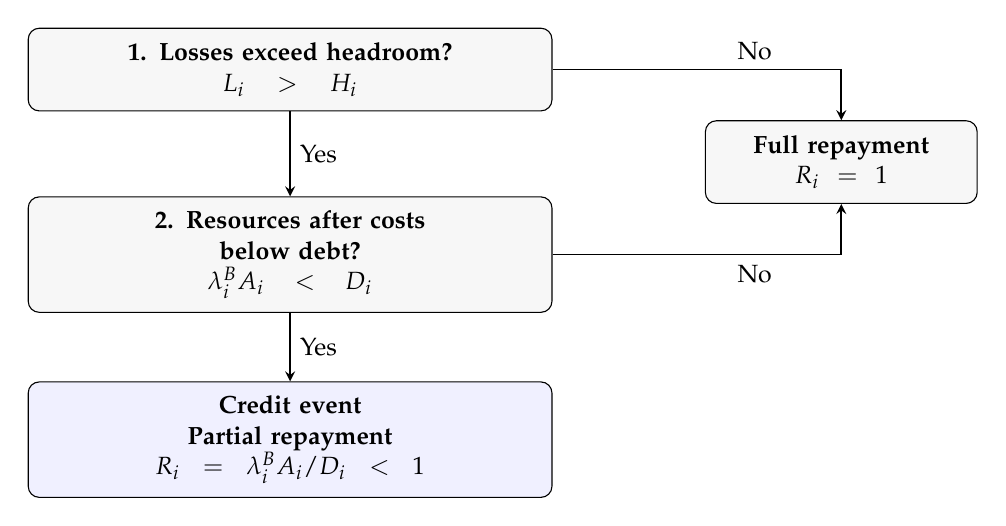
\begin{tikzpicture}[x=1cm,y=1cm,>=stealth,
 test/.style={draw,rounded corners,align=center,text width=6.3cm,minimum height=1.05cm,inner sep=5pt,fill=black!3,font=\small\linespread{1}\selectfont},
 outcome/.style={draw,rounded corners,align=center,text width=6.3cm,minimum height=1.05cm,inner sep=5pt,font=\small\linespread{1}\selectfont}]
 \node[test] (headroom) at (0,0) {\mbox{\textbf{1. Losses exceed headroom?}}\\$L_i>H_i$};
 \node[test] (shortfall) at (0,-2.35) {\textbf{2. Resources after costs}\\\textbf{below debt?}\\$\lambda_i^B A_i<D_i$};
 \node[outcome,fill=blue!6] (partial) at (0,-4.7) {\textbf{Credit event}\\\textbf{Partial repayment}\\$R_i=\lambda_i^B A_i/D_i<1$};
 \node[outcome,text width=3.1cm,fill=black!3] (full) at (7,-1.175) {\textbf{Full repayment}\\$R_i=1$};
 \draw[->,line width=.6pt] (headroom.south) -- node[right,font=\small]{Yes} (shortfall.north);
 \draw[->,line width=.6pt] (shortfall.south) -- node[right,font=\small]{Yes} (partial.north);
 \draw[->,line width=.6pt] (headroom.east) -| node[pos=.35,above,font=\small]{No} (full.north);
 \draw[->,line width=.6pt] (shortfall.east) -| node[pos=.35,below,font=\small]{No} (full.south);
\end{tikzpicture}

\end{figure}


\subsection{Equilibrium and the source of multiplicity}\label{subsec:recovery-wedge}

A banking equilibrium in state $s$ is a vector $\mathbf{R}$ satisfying \eqref{eq:bank_repayment} for every bank, using the receipts generated by that same vector. Write this fixed-point problem as $\mathbf{R}=F_s(\mathbf{R})$. The repayment map $F_s$ is nondecreasing: larger receipts from debtor banks cannot reduce a creditor bank's repayment. Since $F_s$ is nondecreasing and maps $\mathcal K$ into itself, Tarski's fixed-point theorem ensures that a least and a greatest equilibrium exist.\footnote{Under the order that compares repayment rates bank by bank, $\mathcal K=[0,1]^{|\mathcal B|}$ is a complete lattice: every subset has a supremum and an infimum in $\mathcal K$. A nondecreasing map from a complete lattice into itself has a least and a greatest fixed point \citep[Theorem~1]{Tarski1955}. Continuity is not required, so the result applies despite the discontinuities caused by default costs.} Let $\mathcal E_0(s)$ be the set of equilibria without intervention, and write $R_j^e(s)$ for bank $j$'s repayment in equilibrium $e\in\mathcal E_0(s)$. Denote the greatest repayment vector by $\bar{\mathbf{R}}(s)$ and its equilibrium by $e^*(s)$. We call this outcome preferred because it maximizes every bank's repayment, without claiming a welfare ranking. Thus $\bar R_j(s)=R_j^{e^*(s)}(s)$. We call defaults that persist in this greatest-repayment outcome fundamental defaults.

Without default costs ($\lambda_i^B=1$ for every bank), equation~\eqref{eq:bank_repayment} reduces to capped pro-rata repayment, $R_i=\min\{1,A_i/D_i\}$, as in \citet{EisenbergNoe2001}. Total payment is then $D_iR_i=\min\{D_i,A_i\}$: it is continuous in resources, and a one-euro reduction in resources reduces payment by at most one euro. If every bank also owes a positive share of its debt to nonbank creditors, only a fraction of this payment reduction reaches other banks. Together, these two properties make the clearing map a contraction in total payments and imply a unique equilibrium. Deposit funding supplies the outside-creditor condition in the calibration. Appendix~\ref{app:solver_details} gives the proof and relates this condition to Eisenberg and Noe's regularity assumption. The unique equilibrium can still contain bank defaults.

Allowing default costs ($\lambda_i^B<1$) preserves the outside-creditor condition and the monotonicity of the repayment map, but changes the payment rule. Crossing the distress threshold can now trigger a cost on the entire remaining estate: an arbitrarily small reduction in resources can cause a discrete drop in payment. This jump violates the bound on payment changes used in the contraction argument, so outside creditors alone no longer guarantee uniqueness. Continuity alone would not establish uniqueness either; the benchmark argument uses the quantitative bound together with payments to outside creditors. Lower counterparty payments can cause bank defaults even without default costs. The distinction here is that, with default costs, repayment feedback can sustain both a full-repayment equilibrium and an equilibrium with mutually reinforcing bank defaults, for the same exposures and nonbank resources. The following example illustrates this possibility.

\paragraph{A two-bank illustration}
Fix a sovereign state and consider two identical banks. Each owes one unit: half to the other bank and half to nonbank creditors. Each has fixed outside receipts of .51 and the same default-cost parameter $\lambda_i^B=\lambda$. With an accounting-insolvency threshold $T_i=D_i=1$, bank $i$'s assets and repayment are
\[
 A_i=.51+.5R_j,\qquad
 R_i=\begin{cases}1,&A_i\geq1,\\
 \lambda A_i,&A_i<1,\end{cases}\qquad i\ne j.
\]
Without default costs ($\lambda=1$), the unique equilibrium has both banks repaying fully: each receives $A_i=1.01$. With $\lambda=.90$, this equilibrium remains valid, but there is also an equilibrium in which both banks default. Their common repayment solves
\[
 R=.90(.51+.5R),\qquad
 R=\frac{.459}{.55}\simeq.835.
\]
Assets are then approximately .927, below the default threshold, so both defaults are consistent with the repayment rule. The share of debt owed to nonbank creditors remains 50\%: multiplicity arises because repayment jumps from a left limit of .90 to one when assets reach the threshold.

\subsection{Solution}

We solve the clearing system separately for every sovereign state. In each state, we enumerate all bank credit-event sets, solve for the candidate repayment vector associated with each set, and retain every vector that satisfies the original repayment rule. This procedure identifies all equilibria, including the least and greatest repayment vectors; Appendix~\ref{app:solver_details} gives the algorithm. State-by-state equilibria do not require probabilities for sovereign states. These probabilities enter only when computing averages across states.

To distinguish direct losses from repayment feedback, we also identify defaults under full interbank repayment: we apply the sovereign and private-credit losses while assuming that every interbank claim is paid in full, and check which banks breach their distress thresholds. These defaults are caused by direct losses alone. Comparing this diagnostic with equilibrium clearing shows how endogenous repayment shortfalls change bank outcomes. If no bank defaults in this diagnostic, full bank repayment is an equilibrium, but default costs may allow additional equilibria with lower repayments. The diagnostic is a benchmark calculation, not a sequence of settlements.



\section{Calibration}\label{sec:calibration}

The quantitative exercise combines an end-2024 exposure network for Germany (DEU), France (FRA), Italy (ITA) and Spain (ESP) with a sovereign-crisis scenario. The matrix and reported balance sheets determine the positions at risk. Public capital data and the scenario specify when losses trigger costly distress. Appendix~\ref{app:calibration-details} gives the numerical implementation; the Online Appendix documents the source data and reconstruction.

\subsection{The exposure network}

The database combines ECB bank balance sheets and securities holdings, Eurostat financial accounts and International Monetary Fund (IMF) portfolio positions. The choice of a common residence basis is driven by data availability and the need to combine these public sources with consistent institutional coverage. A country's bank block includes banking offices located there, including foreign-owned offices, and excludes offices abroad, including those owned by domestic banking groups. Worldwide consolidated bank data would instead include foreign affiliates whose assets and liabilities fall outside the resident sectors measured by the other sources.

Within this residence-based network, we use public ECB information to estimate and remove loans between offices of the same banking group. We retain the remaining domestic interbank claims without netting them against matching liabilities: each national bank block represents distinct institutions sharing a repayment rate.\footnote{The ECB data report aggregate loan and deposit positions between offices of the same group, rather than a complete bilateral matrix. The Online Appendix explains how we allocate these amounts and remove the corresponding loans where the available data permit. Positions without a public breakdown are not assumed absent. This adjustment does not amount to worldwide group consolidation.} This choice matters for repayment feedback. In an alternative calculation, netting domestic interbank assets against the corresponding liabilities eliminates multiplicity at the reference parameters (Appendix~\ref{app:ocr_robustness}).

The public sources provide totals by instrument and some counterparty detail, but no complete bilateral exposure matrix. We reconstruct missing positions using the available totals and counterparty information, and reconcile discrepancies across sources as documented in the Online Appendix. The results are conditional on this reconstruction.

Sovereign bond holdings are reconciled to official debt-security totals, and household claims on banks comprise deposits and securities holdings. The exposure matrix covers selected instruments; we reconcile it with complete bank balance sheets to obtain repayment resources and clearing debts while retaining full accounting equity. Obligations settled outside the common repayment pool are deducted from both resources and debt.

Figure~\ref{fig:calibrated-exposure-network} isolates the sovereign and interbank exposures at the centre of the spillover mechanism. Arrow widths measure each claim relative to the creditor banking system's reported total assets. Table~\ref{tab:bank-exposures} reports the same positions in amounts and as percentages of total assets, with one column per creditor banking system. Italian and Spanish banks' domestic sovereign holdings stand out, while domestic interbank claims are particularly large in Germany and France. The loops represent claims between distinct banks within a national block. Sovereigns are passive nodes: their repayments depend on the sovereign state, whereas banks' repayments respond to their counterparties. Appendix~\ref{app:calibration-details}, Figure~\ref{fig:full-exposure-network}, shows the broader sector network.

\begin{figure}[t]
\centering
\floatcaption{Bank exposures to sovereigns and banking systems, end-2024}{Arrows run from creditor banks to debtor banks or sovereigns; their widths are proportional to the claim divided by the creditor banking system's reported total assets. All 32 bank--bank and bank--sovereign positions are represented, including very small foreign exposures. Colours identify the creditor's country, as in Figure~\ref{fig:full-exposure-network}. Labels give domestic exposures as percentages of total assets. Loops are domestic claims between distinct institutions after the related-office adjustment. Sovereigns have no outgoing arrows. Other asset classes are omitted from this view; calculations retain the full exposure network.}
\label{fig:calibrated-exposure-network}

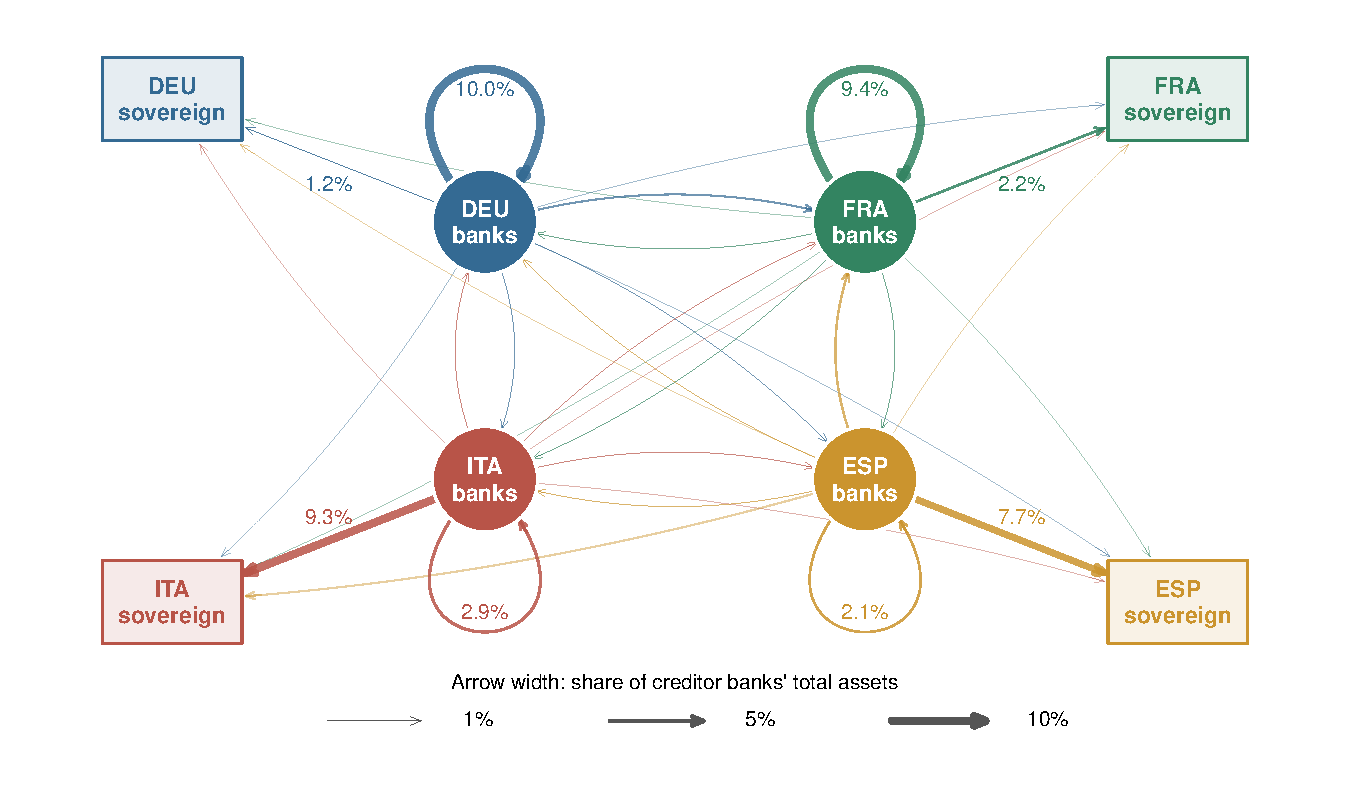
\includegraphics[width=\textwidth]{Figures/bank_exposure_network.pdf}

\end{figure}

\begin{table}[htbp]
\centering
\floatcaption{Bank exposures to sovereigns and banking systems, end-2024}{Columns identify creditor banking systems; rows identify debtor sovereigns or banking systems. Each cell reports EUR billions, followed in parentheses by the percentage of the creditor banking system's reported total assets. The last row gives that denominator in EUR billions. A positive share that rounds to zero at one decimal place is shown as $<0.1\%$. Sovereign exposures are bond holdings; interbank claims include loans and securities after the related-office adjustment. Domestic interbank claims are between distinct institutions. These are the positions shown in Figure~\ref{fig:calibrated-exposure-network}; other assets are outside this table.}
\label{tab:bank-exposures}
\small
\begin{tabular*}{\textwidth}{@{\extracolsep{\fill}}lrrrr@{}}
\toprule
 & Germany & France & Italy & Spain \\
\midrule
\multicolumn{5}{@{}l}{\textit{Sovereign bonds}} \\
Germany & 134.4 (1.2\%) & 0.4 ($<0.1$\%) & 9.8 (0.3\%) & 1.5 ($<0.1$\%) \\
France & 12.1 (0.1\%) & 259.7 (2.2\%) & 26.5 (0.7\%) & 4.3 (0.1\%) \\
Italy & 14.3 (0.1\%) & 8.1 (0.1\%) & 356.8 (9.3\%) & 44.6 (1.4\%) \\
Spain & 10.6 (0.1\%) & 7.5 (0.1\%) & 42.0 (1.1\%) & 236.6 (7.7\%) \\
\addlinespace
\multicolumn{5}{@{}l}{\textit{Claims on banking systems}} \\
Germany & 1,074.8 (10.0\%) & 98.4 (0.8\%) & 13.3 (0.3\%) & 12.8 (0.4\%) \\
France & 151.6 (1.4\%) & 1,103.9 (9.4\%) & 45.2 (1.2\%) & 57.7 (1.9\%) \\
Italy & 23.4 (0.2\%) & 124.7 (1.1\%) & 112.6 (2.9\%) & 24.8 (0.8\%) \\
Spain & 19.6 (0.2\%) & 83.1 (0.7\%) & 10.9 (0.3\%) & 66.4 (2.1\%) \\
\midrule
Total bank assets & 10,801.2 & 11,715.2 & 3,849.0 & 3,092.4 \\
\bottomrule
\end{tabular*}

\end{table}

\subsection{The crisis specification}\label{subsec:calibration_choices}

We set sovereign recovery at 50\% of contractual bond payments, a rounded benchmark consistent with the order of magnitude observed in historical sovereign defaults. Moody's reports an issuer-weighted average recovery rate of 53\% on defaulted sovereign bonds over 1998--2021 \citep{MoodysSovereign2022}.\footnote{Moody's measures recovery using bond trading prices around default or the closing of a distressed exchange; its value-weighted average is lower, at 40\%. Recoveries vary substantially across episodes: the same report records 24\% and 37\% for Greece's two 2012 defaults. These market-value recovery measures motivate the magnitude of our one-period payment assumption, rather than provide an exact estimate for each sample country.}

To turn sovereign bond holdings into repayment resources, we need both the payment following default and the promised payment in its absence. We calibrate the latter using market prices of sovereign default protection: greater default risk implies a higher promised payment, so that each sovereign bond has the same average payoff as the safe asset under these pricing inputs.\footnote{The inputs are derived from sovereign credit default swap (CDS) premiums, the prices paid for protection against sovereign credit events. They reflect market pricing of risk rather than historical default frequencies. Appendix~\ref{app:calibration-details} gives the data, the conversion into default-risk inputs and the payoff formula.} This provides a common pricing benchmark before comparing the losses caused by different sovereign defaults.

The scenario also includes a deterioration in private credit in the country whose sovereign defaults. Using private-credit impairment proxies from the ECB's 2025 bank stress test \citep{ECBStress2025}, we impose losses of 1.8\% on bank loans to firms resident in that country and 1.7\% on bank loans to resident households, regardless of the lending bank's country. These impairments reduce $a_i(s)$, the nonbank repayment resources introduced in Section~\ref{sec:model_banks}, alongside the loss on sovereign bonds. They therefore lower bank resources before interbank repayment feedback and the bank's own default cost. For example, a French sovereign default reduces a German bank's receipts on loans to French firms and households as well as on French government bonds.\footnote{The private-loan loss rates cover a three-year crisis episode and are applied once at settlement. Linking these impairments to the borrower's sovereign-default state is a scenario assumption, not an estimated causal effect. Appendix~\ref{app:calibration-details} gives the exposure mapping and calculations.}

We calibrate bank loss headroom from the capital available above published overall capital requirements (OCR) and leverage requirements, using the ECB's end-2024 selected Pillar 3 disclosures and its Supervisory Banking Statistics for the fourth quarter of 2024 \citep{ECBPublicCapital}. The public supervisory ratios are consolidated, whereas the exposure network is resident-based, so their transfer to national blocks is an explicit proxy. Losses exceeding headroom satisfy the first distress test; they do not mechanically imply legal default or creditor losses. All remaining accounting equity absorbs losses and costs before creditors bear a shortfall. Table~\ref{tab:capital-headroom-summary} summarizes capital ratios and the calibrated buffers by country.

\begin{table}[htbp]
\centering
\floatcaption{Bank capital ratios and loss headroom in amounts and as a share of equity, end-2024}{Percentage headroom is $100H_i/E_i$. CET1 is Common Equity Tier 1 capital; its ratio uses risk-weighted assets as denominator. The leverage ratio divides Tier 1 capital by a regulatory measure of total exposures without risk weights: balance-sheet assets plus exposures from derivatives, securities financing and off-balance-sheet commitments, with regulatory adjustments. Ratios are unweighted bank medians from the ECB Pillar 3 sample (Germany: 23 banks; France: 11; Italy: 12; Spain: 10). Equity covers resident bank blocks; headroom is the country proxy transferred from consolidated-bank capital data, accounting for both capital and leverage requirements. It is not obtained by subtracting a requirement from the displayed median ratios. Sources: \citet{ECBPublicCapital}; calculations and perimeter adjustment in Appendix~\ref{app:calibration-details}.}
\label{tab:capital-headroom-summary}
\small

\begin{tabular*}{\textwidth}{@{\extracolsep{\fill}}lrrrrr@{}}
\toprule
Country & \shortstack{CET1 ratio\\(\%)} & \shortstack{Leverage ratio\\(\%)} & \shortstack{Equity $E_i$\\(EUR bn)} & \shortstack{Headroom $H_i$\\(EUR bn)} & \shortstack{Headroom\\(\% of equity)} \\
\midrule
Germany & 17.7 & 6.8 & 686.4 & 196.8 & 28.7 \\
France & 17.8 & 6.7 & 657.0 & 208.3 & 31.7 \\
Italy & 15.9 & 6.3 & 331.2 & 90.6 & 27.3 \\
Spain & 13.0 & 5.9 & 245.7 & 61.5 & 25.0 \\
\bottomrule
\end{tabular*}

\end{table}


We set $\lambda_i^B=\lambda=.90$ for all bank blocks, a 10\% remaining-estate cost, following the bank-distress modelling benchmark in \citet{Aikman2009}. NBFIs have no additional default cost; their pooled public buffers support full debt repayment. Headroom estimates, the NBFI bound and alternative assumptions are reported in the appendices. Appendix~\ref{app:calibration-details} compares our data coverage, institutional perimeter, contagion channels and bank distress thresholds with those of the ECB's Interconnected System-wide stress test Analytics (ISA) application; the Online Appendix provides further detail.\footnote{ISA uses consolidated bank and fund groups and country-level insurance data, and includes liquidity adjustment, fire-sale price feedback and bank default below a 4.5\% CET1 ratio or following liquidity shortfalls \citep{GrassiEtAl2025}. Our model does not determine how asset sales change market prices and other institutions' asset values. Instead, $1-\lambda_i^B$ captures realization losses and franchise disruption in reduced form. Our baseline distress trigger uses OCR/leverage headroom; Appendix~\ref{app:ocr_robustness}, Table~\ref{tab:ocr-robustness}, reports our sensitivity using headroom above the 4.5\% CET1 floor (the row labelled ``ISA headroom'').}

We solve all sixteen sovereign states before assigning probabilities. Most reported results are state-specific or take maxima across states: equilibrium multiplicity, household repayment gaps and worst-case policy commitment capacities do not require a joint distribution of sovereign defaults. We use independent defaults only for the crisis-conditional average interbank losses and recovery-backstop payments reported in Appendix~\ref{app:ocr_robustness} and the average repayment shortfall in Appendix~\ref{app:calibration-details}, using the market-based marginal risk inputs described above. A sovereign crisis means that at least one sovereign defaults. Appendix~\ref{app:ocr_robustness}, Table~\ref{tab:sovereign-dependence}, checks these backstop averages under positively dependent defaults, preserving the marginal risk inputs and state payoffs. Separately, in a state with multiple banking equilibria, the preferred equilibrium receives weight $1-\rho$ and the other equilibria share total weight $\rho=.20$ equally; a unique equilibrium receives weight one. These weights affect averages, not state-specific equilibria. The same calibration is used throughout; the purchase experiment changes only the specified sovereign-bond and reserve positions.


\section{Multiple banking equilibria in the calibrated network}
\label{sec:multiple-equilibria}

Using the end-2024 network and crisis specification from Section~\ref{sec:calibration}, we quantify the repayment feedback described in Section~\ref{subsec:recovery-wedge}. We examine which sovereign shocks admit multiple banking equilibria and how much bank repayments differ across those equilibria, before tracing the resulting shortfalls to household creditors. All results in this section are without intervention.

\subsection{Defaults under full interbank repayment}

Eight of the sixteen sovereign states admit multiple banking equilibria. These are precisely the states involving French sovereign default: seven have two banking equilibria, and simultaneous default by all four sovereigns has three. The remaining eight states each have a unique banking equilibrium, giving 25 equilibria across the full set of sovereign states.

The diagnostic from Section~\ref{sec:model} identifies defaults under full interbank repayment in twelve states, involving Italian or Spanish banks. Equilibrium repayment feedback also produces French bank defaults in eight states and German bank default in one. Thus the location of defaults caused by direct losses alone does not by itself identify where multiple equilibria arise.

For equilibrium $e$ in sovereign state $s$, define the
aggregate bank-debt recovery rate as
\[
 \mathcal R_B(e,s)
 =\frac{\sum_jD_jR_j^e(s)}{\sum_jD_j},
\]
where $R_j^e(s)$ is bank $j$'s repayment per unit of debt in equilibrium $e$ and sovereign state $s$, determined by equation~\eqref{eq:bank_repayment}.
Table~\ref{tab:bank-recovery-dispersion} reports the range of
$\mathcal R_B(e,s)$ across the banking equilibria of each sovereign state.
It also identifies the banking system with the lowest individual repayment
rate across all banks and equilibria in that state, and gives that same
system's repayment in the preferred equilibrium in parentheses when the state admits multiple equilibria.

\begin{table}[htbp]
\centering
\floatcaption{Dispersion in bank-debt recovery within each sovereign state}{Country codes identify defaulting sovereigns; None denotes no sovereign
default. Equilibria counts banking equilibria without intervention. Aggregate
recovery is the debt-weighted mean repayment rate
$\mathcal R_B(e,s)=\sum_jD_jR_j^e(s)/\sum_jD_j$; its reported range is the
minimum and maximum across $e\in\mathcal E_0(s)$. Lowest bank recovery reports
the country and repayment rate of the banking system with the smallest
$R_j^e(s)$ across all $j$ and $e\in\mathcal E_0(s)$. The parenthesized rate is the repayment of that same banking system in the
preferred equilibrium $e^*(s)$ defined in Section~\ref{subsec:recovery-wedge}. When the equilibrium is unique, the parenthesized rate is omitted and aggregate recovery is reported as a single value. A dash denotes full repayment by all banks in every equilibrium of that state.}
\label{tab:bank-recovery-dispersion}

\begin{tabular*}{\textwidth}{@{\extracolsep{\fill}}lrrl@{}}
\toprule
Sovereign defaults & Equilibria & Aggregate recovery range & Lowest bank recovery \\
\midrule
None & 1 & 100\% & $-$ \\
ESP & 1 & 99.3\% & ESP/93.9\% \\
ITA & 1 & 99.2\% & ITA/94.2\% \\
ITA+ESP & 1 & 98.3\% & ESP/93.0\% \\
FRA & 2 & 97.9\%--100\% & FRA/94.7\% (100\%) \\
FRA+ESP & 2 & 97.2\%--99.3\% & ESP/93.7\% (93.8\%) \\
FRA+ITA & 2 & 97.1\%--99.2\% & ITA/93.7\% (93.8\%) \\
FRA+ITA+ESP & 2 & 96.1\%--98.2\% & ESP/92.8\% (92.9\%) \\
DEU & 1 & 100\% & $-$ \\
DEU+ESP & 1 & 99.3\% & ESP/93.9\% \\
DEU+ITA & 1 & 99.2\% & ITA/94.0\% \\
DEU+ITA+ESP & 1 & 98.3\% & ESP/93.0\% \\
DEU+FRA & 2 & 97.9\%--100\% & FRA/94.7\% (100\%) \\
DEU+FRA+ESP & 2 & 97.2\%--99.3\% & ESP/93.7\% (93.8\%) \\
DEU+FRA+ITA & 2 & 97.0\%--99.2\% & ITA/93.5\% (93.6\%) \\
DEU+FRA+ITA+ESP & 3 & 94.5\%--98.2\% & ITA/92.7\% (92.8\%) \\
\bottomrule
\end{tabular*}

\par\smallskip

\end{table}

\subsection{Two equilibria following a French sovereign default}

To see how these repayment differences arise, consider the state in which only the French sovereign defaults (Figure~\ref{fig:french-default-balance-sheets}). In equilibrium A all banks repay in full. In equilibrium B the French bank block has a credit event, while the other banks still repay in full. French bank repayment falls to 94.7\%, reducing domestic French interbank receipts by EUR~58.2 billion. This extra receipt loss moves total French pre-cost losses above OCR headroom, validating the adverse outcome. The foreign bank blocks lose receipts but do not default.

The adverse French equilibrium retains about EUR~419 billion of pre-cost equity. Its 10\% distress cost is about EUR~841 billion, leaving a creditor shortfall of about EUR~421 billion. The distinction between a prudential trigger and accounting insolvency is therefore consequential.

\begin{figure}[htbp]
\centering
\floatcaption{Partial banking-system balance sheets in the two equilibria following
a French sovereign default}{All amounts are EUR billions. Estate is $A_i$, the total resources available to repay bank debt before distress costs, after fixed outside settlements; it includes remaining equity. Equity is opening accounting equity and Headroom the public OCR loss capacity. B--B means bank-to-bank: claims include domestic claims among distinct institutions, and loss is the reduction in receipts on these claims. Shaded boxes mark credit events. Full remaining equity is included in repayment capacity.}
\label{fig:french-default-balance-sheets}

\begin{tabular*}{\textwidth}{@{\extracolsep{\fill}}llll@{}}
\multicolumn{4}{l}{\textbf{Equilibrium A}} \\
\fcolorbox{black}{white}{\parbox[t]{.212\textwidth}{\centering\scriptsize\textbf{DEU}\par Full repayment\par 100\%\par\smallskip\begin{tabular}{@{}lr@{}}Estate & 8133.6\\
Debt & 7453.6\\
Equity & 686.4\\
Headroom & 196.8\\
B--B claims & 1269.5\\
B--B loss & 0.0\end{tabular}}} & \fcolorbox{black}{white}{\parbox[t]{.212\textwidth}{\centering\scriptsize\textbf{FRA}\par Full repayment\par 100\%\par\smallskip\begin{tabular}{@{}lr@{}}Estate & 8465.2\\
Debt & 7987.6\\
Equity & 657.0\\
Headroom & 208.3\\
B--B claims & 1410.1\\
B--B loss & 0.0\end{tabular}}} & \fcolorbox{black}{white}{\parbox[t]{.212\textwidth}{\centering\scriptsize\textbf{ITA}\par Full repayment\par 100\%\par\smallskip\begin{tabular}{@{}lr@{}}Estate & 3019.0\\
Debt & 2697.1\\
Equity & 331.2\\
Headroom & 90.6\\
B--B claims & 182.0\\
B--B loss & 0.0\end{tabular}}} & \fcolorbox{black}{white}{\parbox[t]{.212\textwidth}{\centering\scriptsize\textbf{ESP}\par Full repayment\par 100\%\par\smallskip\begin{tabular}{@{}lr@{}}Estate & 2661.9\\
Debt & 2415.9\\
Equity & 245.7\\
Headroom & 61.5\\
B--B claims & 161.7\\
B--B loss & 0.0\end{tabular}}} \\
\noalign{\vskip 8pt}
\multicolumn{4}{l}{\textbf{Equilibrium B}} \\
\fcolorbox{black}{white}{\parbox[t]{.212\textwidth}{\centering\scriptsize\textbf{DEU}\par Full repayment\par 100\%\par\smallskip\begin{tabular}{@{}lr@{}}Estate & 8125.6\\
Debt & 7453.6\\
Equity & 686.4\\
Headroom & 196.8\\
B--B claims & 1269.5\\
B--B loss & 8.0\end{tabular}}} & \fcolorbox{black}{black!10}{\parbox[t]{.212\textwidth}{\centering\scriptsize\textbf{FRA}\par Credit event\par 94.7\%\par\smallskip\begin{tabular}{@{}lr@{}}Estate & 8406.9\\
Debt & 7987.6\\
Equity & 657.0\\
Headroom & 208.3\\
B--B claims & 1410.1\\
B--B loss & 58.2\end{tabular}}} & \fcolorbox{black}{white}{\parbox[t]{.212\textwidth}{\centering\scriptsize\textbf{ITA}\par Full repayment\par 100\%\par\smallskip\begin{tabular}{@{}lr@{}}Estate & 3016.7\\
Debt & 2697.1\\
Equity & 331.2\\
Headroom & 90.6\\
B--B claims & 182.0\\
B--B loss & 2.4\end{tabular}}} & \fcolorbox{black}{white}{\parbox[t]{.212\textwidth}{\centering\scriptsize\textbf{ESP}\par Full repayment\par 100\%\par\smallskip\begin{tabular}{@{}lr@{}}Estate & 2658.8\\
Debt & 2415.9\\
Equity & 245.7\\
Headroom & 61.5\\
B--B claims & 161.7\\
B--B loss & 3.0\end{tabular}}} \\
\noalign{\vskip 8pt}
\end{tabular*}


\par\smallskip

\end{figure}


The French example illustrates the repayment gap created by multiplicity within a given sovereign state. The next subsection traces this gap to direct household claims; Section~\ref{sec:ex-post-compensation} then studies creditor compensation and guarantees that change the equilibrium outcome.

\subsection{Household consumption across banking equilibria}
\label{subsec:household-macro-implications}

With portfolios, debt payments and other resources fixed, differences in gross bank receipts give a conditional date-2 consumption equivalent. Let $c_{2,c}^e(s)$ denote country $c$'s household consumption at date 2 in equilibrium $e$ and sovereign state $s$. Relative to the preferred equilibrium $e^*(s)$, the shortfall is
\begin{equation}
 \Delta c_{2,c}^{e}(s)
 =c_{2,c}^{e^*(s)}(s)-c_{2,c}^{e}(s)
 =\sum_{j\in\mathcal B}x_{H_c,j}
   \left[R_j^{e^*(s)}(s)-R_j^e(s)\right].
 \label{eq:household-consumption-shortfall}
\end{equation}
Only bank payments vary across equilibria within a sovereign state in the
baseline. Debt payments and common income cancel in this comparison.

Table~\ref{tab:household-consumption-changes} reports maximum shortfalls by
country and sovereign state, with percentages of observed 2024 consumption
in parentheses. Total is maximized within a single equilibrium. These are
gaps under the same sovereign shock; zero in a unique-equilibrium state
does not imply zero loss from sovereign default.

\begin{table}[htbp]
\centering
\floatcaption{Gross household receipt shortfalls and consumption equivalents}{Country codes in the first column identify defaulting sovereigns;
None denotes no sovereign default. Equilibria counts banking equilibria
without intervention. Country columns report
$\max_{e\in\mathcal E_0(s)}\Delta c_{2,c}^e(s)$; Total reports
$\max_{e\in\mathcal E_0(s)}\sum_c\Delta c_{2,c}^e(s)$, with the sum taken
before maximization. Amounts are rounded to whole EUR billions independently; $<1$ denotes a
positive amount below EUR~1 billion and a dash denotes zero. Parentheses
report percentages of observed 2024 household and non-profit institutions serving households (NPISH) final consumption
expenditure (Eurostat, \texttt{nama\_10\_gdp}, \texttt{P31\_S14\_S15},
current prices; retrieved 21 October 2026). Denominators are EUR~2,359.2 billion
(DEU), 1,595.5 billion (FRA), 1,273.7 billion (ITA), and 883.8 billion (ESP).
Total is divided by their sum. Percentages are calculated from unrounded losses.
Portfolios and nonbank payments are held fixed within each sovereign state. The figures cover direct household bank claims before deposit insurance, compensation, associated financing, indirect ownership and output responses. They are not estimates of uninsured household losses or realized aggregate consumption effects.}
\label{tab:household-consumption-changes}

\begingroup
\small
\setlength{\tabcolsep}{3pt}
\begin{tabular*}{\textwidth}{@{\extracolsep{\fill}}lrrrrrr@{}}
\toprule
Sovereign defaults & Equilibria & DEU & FRA & ITA & ESP & Total \\
\midrule
None & 1 & $-$ & $-$ & $-$ & $-$ & $-$ \\
ESP & 1 & $-$ & $-$ & $-$ & $-$ & $-$ \\
ITA & 1 & $-$ & $-$ & $-$ & $-$ & $-$ \\
ITA+ESP & 1 & $-$ & $-$ & $-$ & $-$ & $-$ \\
FRA & 2 & 1 (0.04\%) & 102 (6.39\%) & $<1$ (0.02\%) & $<1$ (0.01\%) & 103 (1.69\%) \\
FRA+ESP & 2 & 1 (0.04\%) & 104 (6.53\%) & $<1$ (0.02\%) & 1 (0.15\%) & 107 (1.75\%) \\
FRA+ITA & 2 & 1 (0.04\%) & 105 (6.58\%) & 1 (0.11\%) & $<1$ (0.01\%) & 108 (1.76\%) \\
FRA+ITA+ESP & 2 & 1 (0.05\%) & 108 (6.75\%) & 1 (0.11\%) & 1 (0.16\%) & 112 (1.83\%) \\
DEU & 1 & $-$ & $-$ & $-$ & $-$ & $-$ \\
DEU+ESP & 1 & $-$ & $-$ & $-$ & $-$ & $-$ \\
DEU+ITA & 1 & $-$ & $-$ & $-$ & $-$ & $-$ \\
DEU+ITA+ESP & 1 & $-$ & $-$ & $-$ & $-$ & $-$ \\
DEU+FRA & 2 & 1 (0.04\%) & 102 (6.40\%) & $<1$ (0.02\%) & $<1$ (0.01\%) & 103 (1.69\%) \\
DEU+FRA+ESP & 2 & 1 (0.04\%) & 104 (6.54\%) & $<1$ (0.02\%) & 1 (0.15\%) & 107 (1.75\%) \\
DEU+FRA+ITA & 2 & 1 (0.04\%) & 105 (6.59\%) & 1 (0.11\%) & $<1$ (0.01\%) & 108 (1.76\%) \\
DEU+FRA+ITA+ESP & 3 & 124 (5.26\%) & 109 (6.83\%) & 2 (0.15\%) & 2 (0.19\%) & 237 (3.87\%) \\
\bottomrule
\end{tabular*}

\endgroup
\par\smallskip

\end{table}

Following French sovereign default alone, the gross French household receipt gap is EUR~102 billion (6.39\% of observed annual consumption), compared with about EUR~1 billion (0.04\%) in Germany. French bank repayment falls from 100\% to 94.7\%; German banks still repay fully. Because most household bank claims are deposits, translating this gross gap into actual consumption requires information on deposit protection and its financing that the aggregate matrix does not supply.

Section~\ref{sec:ex-post-compensation} studies how a guarantee can eliminate these within-state repayment gaps. Appendix~\ref{app:household-completion} gives an optional household model linking receipts to consumption and utility. The table itself requires no preference calibration and reports gross receipt differences.



\section{From ex post compensation to a credible guarantee}
\label{sec:ex-post-compensation}

A repayment guarantee can interrupt the feedback that sustains an adverse equilibrium. We first measure the losses relative to the highest-repayment outcome, then ask what financial backing makes that outcome unique. Protection is directed to interbank creditors, whose receipts enter bank clearing. Financing is external to the bank block and does not reduce banks' other resources.

\subsection{The preferred outcome and the compensation benchmark}

The preferred equilibrium $e^*(s)$ and its repayment vector $\bar{\mathbf{R}}(s)$ are defined in Section~\ref{subsec:recovery-wedge}. As the greatest fixed point, this vector dominates every other equilibrium and maximizes $\sum_jR_j^e(s)$. It can retain defaults caused by fundamental losses.

Let $L_j^{BB}=\sum_{i\in\mathcal B}x_{ij}$ be bank $j$'s debt to banking creditors, including claims among distinct institutions in the same country. If equilibrium $e$ has already occurred, compensating their shortfall relative to the preferred outcome costs
\[
 C_B(e,s)=\sum_jL_j^{BB}[\bar R_j(s)-R_j^e(s)]_+,
 \qquad [z]_+=\max\{z,0\}.
\]
For example, 40 units of debt repaid at .90 instead of .98 require compensation of $40(.98-.90)=3.2$. Extending compensation to all creditors gives $C_A(e,s)=\sum_jD_j[\bar R_j(s)-R_j^e(s)]_+$. Neither calculation changes the realized repayments.

The largest bank-creditor bill within a state is $C_{B,\max}(s)=\max_{e\in\mathcal E_0(s)}C_B(e,s)$. Its maximum across states defines
\begin{equation}
 B_{\mathrm{post}}=\max_s C_{B,\max}(s),\qquad
 b_{\mathrm{post}}=B_{\mathrm{post}}/\sum_jD_j.
 \label{eq:ex-post-compensation-bound}
\end{equation}
This maximum covers mutually exclusive states; it is not a sum or an expectation. Table~\ref{tab:ex-post-compensation} reports the bills for bank creditors and all creditors. The maximum bank-creditor bill is EUR~126 billion, or 0.61\% of aggregate clearing debt. Unique-equilibrium states have no within-state gap, although fundamental losses can remain.

\begin{table}[htbp]
\centering
\floatcaption{Maximum ex post creditor compensation within each sovereign state}{Country codes identify defaulting sovereigns; None denotes no sovereign
default. Equilibria counts banking equilibria without intervention. Banks only
reports $C_{B,\max}(s)$ and All creditors reports $\max_{e\in\mathcal E_0(s)}C_A(e,s)$,
both as percentages of aggregate bank debt, with the corresponding amounts
in EUR billions in parentheses. Percentages are rounded to two decimal
places; euro amounts are rounded to whole billions from the unrounded
compensation bills. A dash denotes zero compensation.
The largest entry in Banks only
is $b_{\mathrm{post}}$ expressed as a percentage. Transfers cover shortfalls
relative to the preferred equilibrium within the same sovereign state.}
\label{tab:ex-post-compensation}

\begin{tabular*}{\textwidth}{@{\extracolsep{\fill}}lrrr@{}}
\toprule
Sovereign defaults & Equilibria & Banks only & All creditors \\
\midrule
None & 1 & $-$ & $-$ \\
ESP & 1 & $-$ & $-$ \\
ITA & 1 & $-$ & $-$ \\
ITA+ESP & 1 & $-$ & $-$ \\
FRA & 2 & 0.35\% (\euro{}72 bn) & 2.05\% (\euro{}421 bn) \\
FRA+ESP & 2 & 0.36\% (\euro{}73 bn) & 2.11\% (\euro{}434 bn) \\
FRA+ITA & 2 & 0.36\% (\euro{}74 bn) & 2.12\% (\euro{}436 bn) \\
FRA+ITA+ESP & 2 & 0.37\% (\euro{}76 bn) & 2.19\% (\euro{}450 bn) \\
DEU & 1 & $-$ & $-$ \\
DEU+ESP & 1 & $-$ & $-$ \\
DEU+ITA & 1 & $-$ & $-$ \\
DEU+ITA+ESP & 1 & $-$ & $-$ \\
DEU+FRA & 2 & 0.35\% (\euro{}72 bn) & 2.05\% (\euro{}422 bn) \\
DEU+FRA+ESP & 2 & 0.36\% (\euro{}74 bn) & 2.11\% (\euro{}434 bn) \\
DEU+FRA+ITA & 2 & 0.36\% (\euro{}74 bn) & 2.13\% (\euro{}437 bn) \\
DEU+FRA+ITA+ESP & 3 & 0.61\% (\euro{}126 bn) & 3.71\% (\euro{}762 bn) \\
\bottomrule
\end{tabular*}

\par\smallskip

\end{table}


\subsection{A repayment floor before settlement}

After the sovereign state is observed and before banks settle, the facility promises bank creditors at least $\bar R_j(s)$ per unit lent to debtor $j$. Exposures and debts are already in place (Figure~\ref{fig:policy-timing}). If the promise is fully honoured, creditors receive $\widetilde R_j$ and the facility pays $P_j$:
\[
 \widetilde R_j=\max\{R_j,\bar R_j(s)\},\qquad
 P_j=L_j^{BB}[\bar R_j(s)-R_j]_+.
\]
Here $R_j$ is the debtor bank's own repayment under the policy.\footnote{The maximum specifies the guarantee for any candidate repayment vector: $\widetilde R_j=R_j$ when $R_j\geq\bar R_j(s)$, and the facility tops up any shortfall otherwise. Proposition~\ref{prop:greatest-floor} below proves that a fully credible floor yields $R_j=\bar R_j(s)$ in equilibrium. Hence $\widetilde R_j=R_j=\bar R_j(s)$ and transfers are zero; this equality is an equilibrium result, not an assumption in the policy rule.} Transfers go to its creditor banks and increase their receipts; nonbank creditors receive $R_j$. Replacing ordinary interbank receipts with $\widetilde R_j$ therefore changes the clearing equations. Repayments and transfers must be solved jointly.

\begin{figure}[htbp]
\centering
\floatcaption{Timing of the repayment-floor guarantee}{The recovery backstop in
Section~\ref{sec:interbank-recovery-backstop} has the same timing.}
\label{fig:policy-timing}

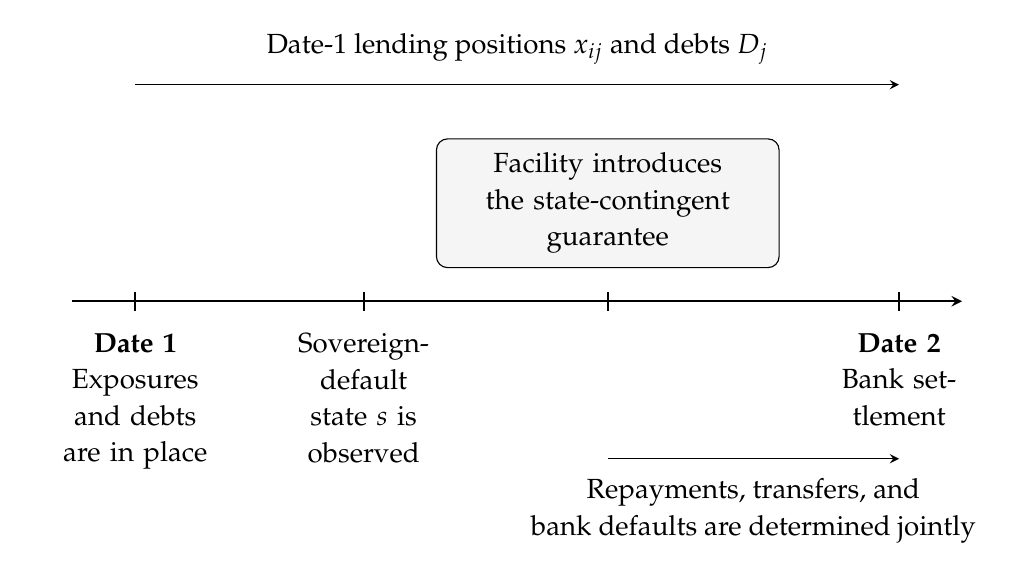
\begin{tikzpicture}[x=1cm,y=1cm,>=stealth,
  event/.style={align=center,text width=2.5cm},
  policy/.style={draw,rounded corners,align=center,text width=4.0cm,
                 inner sep=5pt,fill=black!4}]
  \draw[->,line width=0.7pt] (0,0) -- (11.3,0);
  \foreach \x in {0.8,3.7,6.8,10.5}
    \draw[line width=0.7pt] (\x,-0.12) -- (\x,0.12);

  \node[event,anchor=north] at (0.8,-0.28)
    {\textbf{Date 1}\\Exposures and debts\\are in place};
  \node[event,anchor=north] at (3.7,-0.28)
    {Sovereign-default\\state $s$ is observed};
  \node[policy,anchor=south] at (6.8,0.42)
    {Facility introduces\\the state-contingent\\guarantee};
  \node[event,anchor=north] at (10.5,-0.28)
    {\textbf{Date 2}\\Bank settlement};

  \draw[->,line width=0.5pt] (0.8,2.75) -- (10.5,2.75)
    node[midway,above=5pt,fill=white,inner sep=2pt,align=center]
    {Date-1 lending positions $x_{ij}$ and debts $D_j$};
  \draw[->,line width=0.5pt] (6.8,-2.00) -- (10.5,-2.00)
    node[midway,below=5pt,fill=white,inner sep=2pt,align=center]
    {Repayments, transfers, and\\bank defaults are determined jointly};
\end{tikzpicture}

\end{figure}

\subsection{Unique implementation and sufficient backing}
\label{sec:floor-equilibrium-effects}\label{sec:floor-sufficient-budget}

The repayment floor introduced above promises bank creditors at least the preferred-equilibrium repayment $\bar R_j(s)$ on each debtor bank. Unlike the ex post compensation calculation, this promise enters the clearing equations: protected interbank receipts increase the resources available for banks' own repayments. The question is whether this change merely reduces shortfalls or rules out the adverse equilibria altogether.

With the greatest original repayment vector $\bar{\mathbf{R}}(s)$ as target, the policy equation is $\mathbf{R}=F_s(\mathbf{R}\vee\bar{\mathbf{R}}(s))$, where $\vee$ denotes the componentwise maximum. Proposition~\ref{prop:greatest-floor} shows that, when the promise is credible, this equation has the unique solution $\mathbf{R}=\bar{\mathbf{R}}(s)$. Hence $\mathbf{R}\vee\bar{\mathbf{R}}(s)=\mathbf{R}=\bar{\mathbf{R}}(s)$: banks themselves deliver the target repayments and the facility makes no transfers. This is the coordination role of a credible guarantee \citep{DiamondDybvig1983,JacksonPernoud2021}. For now, we assume the promise is fully honoured; the financial capacity needed to support it is considered after the proposition.

\begin{proposition}[Unique equilibrium under a fully credible floor]\label{prop:greatest-floor}
Fix a sovereign state $s$, portfolios, nonbank receipts and bank repayment rules. Suppose the ordinary repayment map $F_s$ is a nondecreasing self-map of $\mathcal K=[0,1]^{|\mathcal B|}$, and let $\bar{\mathbf{R}}(s)$ be its greatest fixed point. A credible interbank repayment floor at $\bar{\mathbf{R}}(s)$, financed without reducing any bank's other resources, has the unique ordinary repayment vector $\mathbf{R}=\bar{\mathbf{R}}(s)$ and entails zero transfers in equilibrium.
\end{proposition}
\begin{proof}
At any policy equilibrium, monotonicity implies
\[
 \mathbf{R}=F_s(\mathbf{R}\vee\bar{\mathbf{R}})\geq F_s(\bar{\mathbf{R}})=\bar{\mathbf{R}}.
\]
Here and below, inequalities between repayment vectors hold componentwise. Consequently $\mathbf{R}\vee\bar{\mathbf{R}}=\mathbf{R}$, so $\mathbf{R}=F_s(\mathbf{R})$ is an original equilibrium. Since $\bar{\mathbf{R}}$ is its greatest fixed point, $\mathbf{R}\leq\bar{\mathbf{R}}$. Hence $\mathbf{R}=\bar{\mathbf{R}}$. Conversely, $\bar{\mathbf{R}}$ satisfies the policy equation with no transfer.
\end{proof}

The argument has two steps. Protected receipts ensure that every bank can repay at least as much as in the original preferred equilibrium. At such repayments no guarantee is needed, so any policy equilibrium must also be an equilibrium of the original system. Since the preferred equilibrium already has the greatest original repayments, it is the only possibility. Monotonicity is sufficient for this argument; continuity and Eisenberg--Noe regularity are not required.

In the French-only sovereign-default example, the original French bank repayments are 100\% and 94.7\%. The fully credible floor at 100\% changes banks' interbank receipts and eliminates the 94.7\% outcome: French banks themselves repay fully, with no payment by the facility. The result does not eliminate fundamental defaults. If the target includes partial repayment, as for Italian banks after Italian sovereign default alone, that partial repayment remains.

Zero equilibrium transfers do not mean that the promise requires no financial backing. Proposition~\ref{prop:greatest-floor} assumes full credibility without determining the capacity needed to sustain it. Let $B\geq0$ denote the facility's capacity. Recall that $B_{\mathrm{post}}$, defined in equation~\eqref{eq:ex-post-compensation-bound}, is the largest ex post compensation bill for bank creditors, measured relative to the preferred outcome and maximized across the original equilibria and sovereign states. The Online Appendix shows that total guarantee claims at any policy equilibrium cannot exceed $B_{\mathrm{post}}$. Capacity $B\geq B_{\mathrm{post}}$ therefore allows the facility to honour the floor in every policy equilibrium, making the preferred outcome unique by Proposition~\ref{prop:greatest-floor}. Thus the ex post compensation bill provides a sufficient commitment bound. The next subsection asks whether a smaller capacity can also make the preferred equilibrium unique, accounting for how creditors anticipate rationing.

\subsection{Minimum capacity under proportional rationing}\label{sec:minimum-floor-budget}

We fix the allocation rule: when claims exceed capacity $B$, every claimant receives the same fraction of its claim. Let $\mathbf{h}_s(\mathbf{R})=[\bar{\mathbf{R}}(s)-\mathbf{R}]_+$ be the vector of per-unit guarantee claims, with the positive part taken componentwise, and let $H_s(\mathbf{R})=\sum_jL_j^{BB}h_{s,j}(\mathbf{R})$ be their total amount. The paid fraction is $\theta_B(\mathbf{R};s)=\min\{1,B/H_s(\mathbf{R})\}$ for positive claims, and one when claims are zero. Creditors anticipate this fraction, giving
\[
 \mathbf{R}=G_{s,B}(\mathbf{R}):=F_s\bigl(\mathbf{R}+\theta_B(\mathbf{R};s)\mathbf{h}_s(\mathbf{R})\bigr).
\]
To find the critical capacity, consider equilibria at a fixed paid fraction $\theta<1$ with positive total guarantee claims:
\[
 \Gamma_s=\{(\theta,\mathbf{R}):0\leq\theta<1,\ \mathbf{R}\in\mathcal K,\ H_s(\mathbf{R})>0,\
 \mathbf{R}=F_s(\mathbf{R}+\theta \mathbf{h}_s(\mathbf{R}))\}.
\]
Each pair is an adverse outcome because the target has zero claims. Its expenditure is $\theta H_s(\mathbf{R})$; the supremum of these expenditures determines the threshold for unique implementation.

\begin{proposition}[Critical capacity for the proportional floor]\label{prop:critical-floor-budget}
Under the assumptions of Proposition~\ref{prop:greatest-floor}, define
\[
 B_s^\dagger=\sup_{(\theta,\mathbf{R})\in\Gamma_s}\theta H_s(\mathbf{R}),
 \qquad B^\dagger=\max_s B_s^\dagger,
\]
with $B_s^\dagger=0$ if $\Gamma_s$ is empty. In state $s$, every $B>B_s^\dagger$ implements $\bar{\mathbf{R}}(s)$ uniquely, whereas every $0\leq B<B_s^\dagger$ admits another equilibrium. At $B=B_s^\dagger$, uniqueness holds exactly when no pair in $\Gamma_s$ attains the supremum. The target remains an equilibrium with zero transfers at every capacity. Moreover, $B^\dagger\leq B_{\mathrm{post}}$.
\end{proposition}


The Online Appendix proves this characterization and explains how we evaluate it numerically by enumerating possible sets of defaulting banks. The guarantee rule is held fixed: the proposition does not optimize arbitrary capital injections or guaranteed links. The distinction between a critical threshold and an attained minimum matters because the distress rule can jump at equality.

In the calibration, equality implements uniquely in every state. The minimum common capacity is EUR~60.6 billion, or 0.29\% of aggregate clearing debt, 52\% below the sufficient compensation bound. The binding state has all four sovereigns defaulting. Table~\ref{tab:minimum-floor-budget} reports the state thresholds. At these capacities, every surviving outcome equals the original preferred equilibrium and transfers are zero.

\begin{table}[htbp]
\centering
\floatcaption{Minimum capacity of the proportional repayment floor and sufficient compensation bound (EUR billions)}{The matrix, OCR headroom, full accounting equity and $\lambda=.90$ are held fixed. Minimum capacities are evaluated from every admissible default regime; equality at the threshold implements uniquely under the maintained full-repayment convention. Amounts are rounded to one decimal place; comparisons and endpoint tests use unrounded values. All implementing capacities yield zero equilibrium transfers.}
\label{tab:minimum-floor-budget}

\begin{tabular*}{\textwidth}{@{\extracolsep{\fill}}lrr@{}}
\toprule
Sovereign defaults & Minimum capacity & Sufficient bound \\
\midrule
FRA & 31.7 & 71.7 \\
FRA+ESP & 42.9 & 73.5 \\
FRA+ITA & 46.6 & 74.0 \\
FRA+ITA+ESP & 59.8 & 76.2 \\
DEU+FRA & 32.2 & 71.7 \\
DEU+FRA+ESP & 43.4 & 73.6 \\
DEU+FRA+ITA & 47.4 & 74.1 \\
DEU+FRA+ITA+ESP & 60.6 & 126.3 \\
\midrule
Other eight states & 0 & 0 \\
\bottomrule
\end{tabular*}


\end{table}


These are commitment requirements, not estimates of welfare or fiscal cost. Their zero equilibrium disbursements also differ from injections that are paid and later recovered. A guarantee anticipated before exposures were formed could change saving, borrowing and investment; the fixed-exposure result and calibrated capacities do not cover those responses. We next consider a backstop whose protection depends on observed recovery losses, without a preferred-equilibrium target.


\section{A recovery backstop for interbank contagion}
\label{sec:contingent_support}\label{sec:interbank-recovery-backstop}

Section~\ref{sec:ex-post-compensation} guarantees repayments relative to the original preferred equilibrium. We now consider protection defined directly from losses at settlement: the facility covers a fraction of the repayment capacity destroyed by bank default costs. We ask the same two questions: does this rule eliminate adverse equilibria, and what financial resources does it require? Timing and external financing are unchanged.

\subsection{The recovery-backstop rule and clearing}\label{subsec:interbank_recovery_backstop}

Let $\eta\in[0,1]$ be the fraction of default-cost losses covered. For a defaulting bank $j$, ordinary repayment is $R_j=\lambda_j^BA_j/D_j$. Its bank creditors receive
\begin{equation}
 \widehat R_j(s;\eta)=\min\left\{1,
 R_j+\eta\left[A_j/D_j-R_j\right]\right\}.
 \label{eq:interbank_backstop_repayment}
\end{equation}
For a nondefaulting bank, $\widehat R_j=1$; nonbank creditors receive ordinary repayment. The cap prevents overpayment when prudential distress occurs with positive pre-cost equity. At full coverage, bank creditors receive pre-cost repayment capacity capped at par; any fundamental asset shortfall remains uncovered.


Bank resources use guaranteed receipts on interbank claims:
\begin{equation}
 A_i(s)=a_i(s)+\sum_{j\in\mathcal B}x_{ij}\widehat R_j(s;\eta).
 \label{eq:interbank_backstop_assets}
\end{equation}
Together with \eqref{eq:bank_repayment}, this determines bank defaults and repayments jointly. As with the repayment floor, protection changes creditor banks' receipts and therefore their own repayment capacity. Here the protection is tied to the debtor's default-cost loss, rather than to a preferred-equilibrium target.

\subsection{Effects on banking equilibria}

We solve the policy clearing system for all sixteen sovereign states, varying common coverage from 0\% to 100\% in five-percentage-point steps. Multiplicity falls from eight states without intervention to six at 25\% coverage, two at 30\% and one at 35\%. At 40\% and every higher tested coverage, all states have a unique banking equilibrium (Figure~\ref{fig:interbank_recovery_backstop_grid}, panel a).\footnote{At each coverage we enumerate all banking equilibria using the solver in Appendix~\ref{app:solver_details}. A finer sweep in one-percentage-point steps first finds uniqueness in all states at 36\%. These sweeps identify sufficient coverage levels, rather than a minimum over continuous coverage as characterized for the repayment floor in Section~\ref{sec:minimum-floor-budget}.}

The backstop therefore also removes multiplicity in this calibration. It does not generally deliver full repayment: fundamental Italian and Spanish bank credit events can persist. These equilibrium results are obtained state by state and require no probabilities over sovereign states or weights over banking equilibria.

\subsection{Payments required by the backstop}

For policy equilibrium $e$ in state $s$, let $R_j^e(s)$ denote ordinary repayment and $\widehat R_j^e(s;\eta)$ the protected rate. The facility pays
\begin{equation}
 K(e,s;\eta)=\sum_jL_j^{BB}[\widehat R_j^e(s;\eta)-R_j^e(s)]_+.
 \label{eq:interbank_backstop_cost}
\end{equation}
To assess the largest payment requirement, we maximize $K(e,s;\eta)$ over all policy equilibria and sovereign states, as in the compensation benchmark of Section~\ref{sec:ex-post-compensation}. Panel b of Figure~\ref{fig:interbank_recovery_backstop_grid} reports this maximum as a percentage of aggregate bank debt. It requires no probability or equilibrium-selection weights.

At 40\% coverage, the largest payment is EUR~19.3 billion, or 0.09\% of bank debt. At the round half-coverage benchmark it is EUR~24.2 billion, or 0.12\%. Unlike the repayment floor at its target, the recovery backstop can make payments in the surviving equilibrium because it protects creditors against default-cost losses that remain after multiplicity has been eliminated. These amounts are disbursements under the recovery rule; Section~\ref{sec:minimum-floor-budget}'s EUR~60.6 billion is backing for a different promise, which makes no equilibrium transfers.

Panel b is non-monotone because higher coverage both increases reimbursement for continuing bank defaults and can eliminate costly default equilibria. At 35\% coverage, the maximum payment is about EUR~67 billion in the all-sovereign-default state, in an adverse equilibrium that includes French bank default. At 40\%, that equilibrium has disappeared; the maximum shifts to the Italian-and-Spanish sovereign-default state and falls to EUR~19.3 billion. Payments then rise with coverage of the remaining defaults, until the cap on creditor receipts binds.

Appendix~\ref{app:ocr_robustness} reports average losses and payments conditional on a sovereign crisis, together with their sensitivity to sovereign dependence and equilibrium-selection weights. Those averages summarize the distribution of outcomes; they are not used to establish the equilibrium effects or maximum payment requirements above.

\begin{figure}[tp]
\centering
\floatcaption{Equilibrium effects and maximum payments of the common recovery backstop}{Coverage varies in five-percentage-point steps. Panel (a) counts sovereign states with multiple banking equilibria. Panel (b) gives the largest facility payment across all sovereign states and policy equilibria, as a percentage of aggregate clearing debt. Both panels are independent of sovereign probabilities and equilibrium-selection weights. Creditor receipts are capped at par.}
\label{fig:interbank_recovery_backstop_grid}

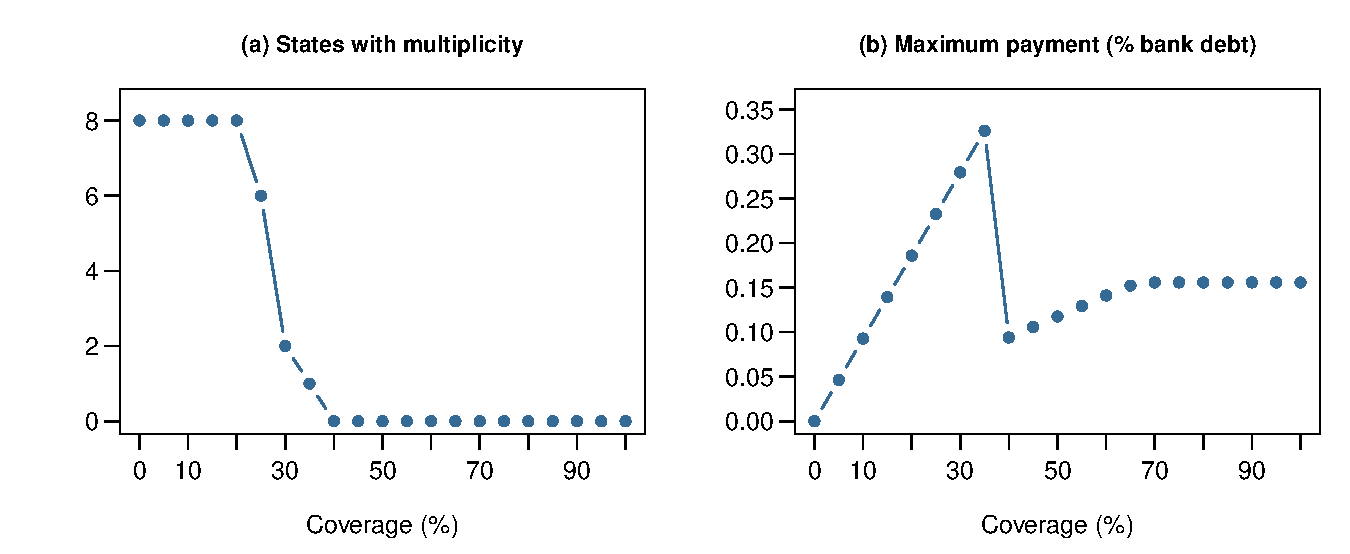
\includegraphics[width=\linewidth]{Figures/interbank_recovery_backstop_grid.pdf}

\end{figure}

\FloatBarrier


\section{Eurosystem purchases of sovereign bonds}\label{sec:eurosystem-purchases}

Guarantees support repayment after the sovereign shock. Bond purchases instead change banks' exposure before it occurs. We consider Eurosystem purchases of bank-held sovereign bonds at the model's date-1 book value of one, with selling banks receiving an equal amount of safe reserves. Such purchases create reserves on bank balance sheets \citep{ECBReserves2021}.

Each experiment specifies the sovereign issuers whose bonds are purchased and a common purchase fraction. For each selected issuer, the Eurosystem buys the stated fraction of the bonds held by each of the four country banking blocks, so purchases across banks are proportional to existing holdings. For example, purchasing 50\% of French holdings means buying half of the French sovereign bonds held by each German, French, Italian and Spanish bank block, while leaving their other sovereign holdings unchanged. In the all-issuer experiments, the stated fraction applies to holdings of all four sovereigns.

Let $P_{ig}\in[0,x_{i,G_g}]$ be the amount of sovereign $g$'s bonds purchased from bank $i$. The bank's direct resource gain in state $s$, holding other banks' repayments fixed, is
\[
 \Delta A_i(s)=\sum_gP_{ig}[1-R_g^G(s)].
\]
Replacing a defaulting sovereign claim with reserves reduces the bank's initial loss. The resulting change in interbank receipts can also remove adverse clearing outcomes. Sovereign debt outstanding is unchanged: the Eurosystem holds the sold bonds and issues the corresponding reserve liabilities. Bank total assets, debt, accounting equity, headroom and private-credit losses remain fixed; prices and credit supply do not respond. Appendix~\ref{app:purchase-implementation} gives the allocation and balance-sheet details.

\subsection{Purchase composition and banking outcomes}

Table~\ref{tab:eurosystem-purchases} compares purchase sizes and issuer compositions. For each experiment, we solve the altered network in every sovereign state and recompute the minimum repayment-floor capacity.

\begin{table}[htbp]
\centering
\floatcaption{Sovereign bond purchases and banking equilibria}{Amounts are EUR billions. Purchases replace bank-held sovereign bonds with safe reserves before the shock at book value. Defaults under full interbank repayment are evaluated after sovereign and private-credit losses, assuming that every interbank claim is paid in full; the two state-count columns range from zero to sixteen. Equilibria is the total across those states. Floor capacity is the attained minimum common capacity under proportional rationing for the post-purchase network; a dash denotes zero. Purchase principal is an asset exchange, not a fiscal cost. All other calibration inputs are unchanged.}
\label{tab:eurosystem-purchases}

\small
\renewcommand{\arraystretch}{1.12}
\begin{tabularx}{\textwidth}{@{}>{\raggedright\arraybackslash}Xrrrrr@{}}
\toprule
Purchased holdings & \shortstack{Purchase\\principal} & \shortstack{Default states\\under full\\interbank repayment} & \shortstack{Multiple\\states} & Equilibria & \shortstack{Floor\\capacity} \\
\midrule
No purchases & $-$ & 12 & 8 & 25 & 60.6 \\
All issuers: 25\% & 292 & 12 & 6 & 22 & 14.2 \\
All issuers: 50\% & 585 & 12 & 0 & 16 & $-$ \\
All issuers: 75\% & 877 & 0 & 0 & 16 & $-$ \\
France only: 50\% & 151 & 12 & 0 & 16 & $-$ \\
Italy and Spain: 75\% & 540 & 0 & 8 & 27 & 39.6 \\
\bottomrule
\end{tabularx}


\end{table}

Purchasing 25\% of banks' sample-country sovereign holdings, EUR~292 billion, reduces multiple states from eight to six and minimum floor capacity from EUR~60.6 billion to EUR~14.2 billion. Purchasing 50\%, EUR~585 billion, eliminates multiplicity while defaults under full interbank repayment remain in twelve states. At 75\%, EUR~877 billion, every banking equilibrium is fully performing.

Issuer composition gives the sharper distinction. Half of banks' French sovereign holdings, EUR~151 billion, suffices to eliminate multiplicity without changing the defaults under full interbank repayment. These purchases weaken the French repayment feedback supporting adverse outcomes. Purchasing three quarters of Italian and Spanish holdings, EUR~540 billion, instead makes full bank repayment an equilibrium in every sovereign state, but leaves eight states with additional equilibria in which banks default. In those adverse outcomes, reduced interbank receipts sustain the defaults, including through domestic interbank claims. Minimum floor capacity remains EUR~39.6 billion. Making full repayment possible and eliminating adverse equilibria are distinct objectives; equilibrium counts need not decline monotonically with purchases.

\subsection{Risk transfer and policy interpretation}

The bank resource gain is matched by a cash shortfall on the Eurosystem's new assets relative to its reserve liabilities. With half of French holdings purchased, the largest additional shortfall across sovereign states is about EUR~75 billion. This is a contingent public exposure, not an expected fiscal cost. The model does not allocate Eurosystem losses among national central banks or feed their financing back to households and sovereigns.

Purchases can therefore interrupt repayment feedback, but transfer sovereign risk to the central bank. The repayment floor can instead eliminate adverse outcomes without equilibrium transfers. Purchase principal and guarantee capacity measure different commitments and cannot establish a fiscal-cost ranking. The exercise isolates exposure reallocation, complementing the valuation and lending channels discussed in the introduction.



\section{Conclusion}\label{sec:conclusion}

A given sovereign shock can support different banking outcomes because repayment shortfalls reinforce one another through financial claims. Default costs permit this feedback even with substantial nonbank funding, separating unavoidable losses from those sustained by multiplicity.

A floor at the greatest original equilibrium removes adverse outcomes without equilibrium transfers. Its credibility requires financial capacity; we characterize the minimum under proportional rationing. A recovery backstop also removes multiplicity but entails payments.

Bond purchases exchange banks' sovereign holdings for safe reserves and transfer risk to the Eurosystem. Our calibration separates purchases that make full bank repayment an equilibrium from those that make the equilibrium unique. Purchase principal and guarantee capacity measure different commitments; neither estimates fiscal cost.

Results depend on distress thresholds, default costs and gross domestic interbank claims, conditional on the reconstructed network. Guarantee financing does not reduce bank resources. Endogenous lending, deposit protection and financing incidence would connect these repayment effects to broader consumption and welfare outcomes.


\clearpage
\setcounter{section}{0}

\begin{center}
\begin{large}

{\bf--- Appendix ---}

\end{large}

\end{center}


\vspace{1cm}


\setcounter{subsection}{0}
\setcounter{equation}{0}
%\renewcommand{\thesection}{O.\arabic{section}}

\appendix
\counterwithin{figure}{section}
\counterwithin{table}{section}
\renewcommand{\thesection}{\Alph{section}}
\renewcommand{\thesubsection}{\thesection.\arabic{subsection}}
\renewcommand{\theequation}{\thesection.\arabic{equation}}
\renewcommand{\thetable}{\thesection.\arabic{table}}
\renewcommand{\thefigure}{\thesection.\arabic{figure}}

\section{Numerical implementation of the equilibrium solver}\label{app:solver_details}

The equilibrium solver works in EUR billions and includes the full accounting estate. Let $\mathbf{B}=(x_{ij})_{i,j\in\mathcal B}$ be the bank claim matrix, $\mathbf{D}=(D_i)$ the clearing-debt vector, and $\mathbf{a}(s)=(a_i(s))$ the net nonbank-resource vector from Section~\ref{sec:model_banks}. All $a_i(s)$ are strictly positive in the calibration. The cutoff $T_i$ is defined in the same section. Appendix~\ref{app:calibration-details} explains how these resources and debts are reconciled to the data. The NBFI balance-sheet check establishes par repayment in this calibration; an independent eight-node enumeration verifies selected results with endogenous NBFIs.

\paragraph{Uniqueness without default costs}
At $\lambda_i^B=1$, write total bank payments as $p_i=D_iR_i$ and define the internal liability shares $\Pi_{ij}=B_{ji}/D_i$: rows are debtors and columns creditors. Collect these shares in $\boldsymbol{\Pi}=(\Pi_{ij})$ and payments in $\mathbf{p}=(p_i)$, with transpose denoted by $\top$. The bank-only clearing map is
\[
 \Psi_s(\mathbf{p})=\min\{\mathbf{D},\mathbf{a}(s)+\boldsymbol{\Pi}^\top \mathbf{p}\},
\]
The minimum is componentwise. The debt share owed within the bank block is $\ell_i=\sum_j\Pi_{ij}$. If $\ell_i<1$ for every bank, some payment from every bank goes to outside creditors. For any two payment vectors $\mathbf{p},\mathbf{p}'$, the $\ell_1$ norm satisfies
\[
 \|\Psi_s(\mathbf{p})-\Psi_s(\mathbf{p}')\|_1
 \leq\|\boldsymbol{\Pi}^\top(\mathbf{p}-\mathbf{p}')\|_1
 \leq\left(\max_i\ell_i\right)\|\mathbf{p}-\mathbf{p}'\|_1.
\]
Thus the map is a contraction and the clearing vector is unique for every nonnegative $\mathbf{a}(s)$. This is a strong sufficient condition for the open bank block, not a necessary condition. Internal debt shares are 16.1\%, 17.0\%, 10.6\% and 7.4\% for Germany, France, Italy and Spain, giving a contraction factor below .18. Clearing debt here excludes fixed outside settlements but retains the nonbank creditors sharing ordinary bank repayment. Gross domestic bank claims remain internal to $\boldsymbol{\Pi}$. With default costs, the map remains contractive within each fixed default regime, but jumps between regimes can prevent global contraction.

\paragraph{Regularity in the original clearing model}
Conditional on a sovereign state and fixed nonbank receipts, the no-cost model has fixed nominal debts, proportional sharing, debt priority over equity and no value destruction at default. Monotonicity gives existence; uniqueness requires an additional condition. In the closed-network formulation of \citet{EisenbergNoe2001}, regularity requires every node's risk orbit---the node and its direct or indirect creditors---to contain positive external resources. Strictly positive external resources at every node are a simple sufficient condition.\footnote{See their Definitions 2--5 and Theorem 2. Paths follow liabilities from debtor to creditor, the reverse of the creditor-to-debtor arrows in our exposure figure. These are sufficient conditions, not necessary conditions for uniqueness.} This excludes closed payment circuits with no external resources to anchor settlement. For example, if two banks owe one unit to each other, have no outside assets and owe nothing outside the pair, any common payment between zero and one clears their obligations. A cycle of obligations can therefore admit indeterminate payments when it has no external anchor. The outside-creditor condition above provides a direct contraction argument for our open bank block; its fixed net external receipts are also positive in all sixteen states.

\paragraph{Default-set enumeration}

For each of sixteen sovereign states, enumerate the sixteen bank default sets $J\subseteq\mathcal B$, with complement $J^c=\mathcal B\setminus J$. The operator $\operatorname{diag}$ forms a diagonal matrix. Subscripts on vectors and matrices select the indicated banks; $\mathbf1$ is a vector of ones and $\mathbf{I}$ an identity matrix of matching dimension. With $\boldsymbol{\Gamma}_J=\operatorname{diag}(\lambda_i^B/D_i)_{i\in J}$, ordinary repayment solves
\[
 [\mathbf{I}-\boldsymbol{\Gamma}_J\mathbf{B}_{JJ}]\mathbf{R}_J
   =\boldsymbol{\Gamma}_J[\mathbf{a}_J(s)+\mathbf{B}_{J,J^c}\mathbf1].
\]
Retain a solution only if $0\leq R_i<1$ and $A_i<T_i$ for $i\in J$, while $R_i=1$ and $A_i\geq T_i$ otherwise. The default check is prudential, not a check that accounting equity is exhausted. Equality belongs to full repayment. Enumeration requires nonsingular candidate systems; the implementation reports an error if this condition fails.

\paragraph{Policy regions}
Let $\eta_j$ denote the backstop coverage assigned to debtor $j$: common coverage $\eta$ for eligible banks and zero for excluded banks. Effective creditor repayment is $\max\{R_j,\bar R_j(s)\}$ under a floor and $\min\{1,\mu_jR_j\}$ on the default branch under a recovery backstop, where $\mu_j=1+\eta_j(1-\lambda_j^B)/\lambda_j^B$. In each binding-floor or binding-cap region, write creditor repayment $d_j+\gamma_jR_j$, where $d_j$ and $\gamma_j$ are that region's intercept and slope. Collect the intercepts in $\mathbf{d}=(d_j)$ and let $\boldsymbol{\gamma}_J=(\gamma_j)_{j\in J}$. The candidate system is
\begin{equation}
 [\mathbf{I}-\boldsymbol{\Gamma}_J\mathbf{B}_{JJ}\operatorname{diag}(\boldsymbol{\gamma}_J)]\mathbf{R}_J
    =\boldsymbol{\Gamma}_J[\mathbf{a}_J(s)+\mathbf{B}_{J,\mathcal B}\mathbf{d}],
 \label{eq:interbank_backstop_linear_system}
\end{equation}
where $\mathbf{a}(s)$ is the fixed external receipt vector defined above. Nondefaulting debtor entries have slope zero and intercept one. Enumerate every region and check its floor/cap inequalities and the original repayment map. Identical boundary roots are counted once. Zero floors and zero backstop coverage reproduce the baseline.

The preferred equilibrium maximizes summed ordinary repayments and is the greatest fixed point of the monotone map. Proposition~\ref{prop:greatest-floor} ensures that the floor leaves exactly that equilibrium and pays zero; enumeration verifies this in every state. Proposition~\ref{prop:critical-floor-budget} characterizes the critical capacity of the proportional capped floor. The online appendix gives its proof and the finite default-regime calculation, including the endpoint test. Expected results assign weight $1-\rho$ to the highest-sum repayment root and share $\rho$ equally among other roots, using $\rho=.20$ for the reference; unique states receive weight one. Sovereign-state probabilities are products of the calibrated default/survival probabilities.

\section{Data, accounting and calibration}\label{app:database_construction}\label{app:calibration-details}

\subsection{Source coverage and balance-sheet reconciliation}

The Online Appendix explains the public source hierarchy, missing bilateral allocations and the treatment of related offices. The 24-account reporting matrix preserves the rest of the world and unidentified holders and issuers separately. The model groups them into Other counterparties without netting claims; the Eurosystem remains separate. Figure~\ref{fig:full-exposure-network} shows the resulting 22-node network, complementing the bank-focused view in Section~\ref{sec:calibration}. Figure~\ref{fig:active_source_matrix} records source coverage.

\begin{figure}[htbp]
\centering
\floatcaption{Residence-based exposure network, end-2024}{Bk = banks; Gvt = government; NBFI = nonbank financial institutions; Firm = firms; HH = households. Arrows run from creditor to debtor and retain the five largest outgoing claims per node; calculations use the full network. Thickness increases with the claim size in EUR billions. Colours identify countries or aggregate blocks. Gross domestic bank claims are retained in clearing but omitted from this drawing; Figure~\ref{fig:calibrated-exposure-network} displays them as loops.}
\label{fig:full-exposure-network}
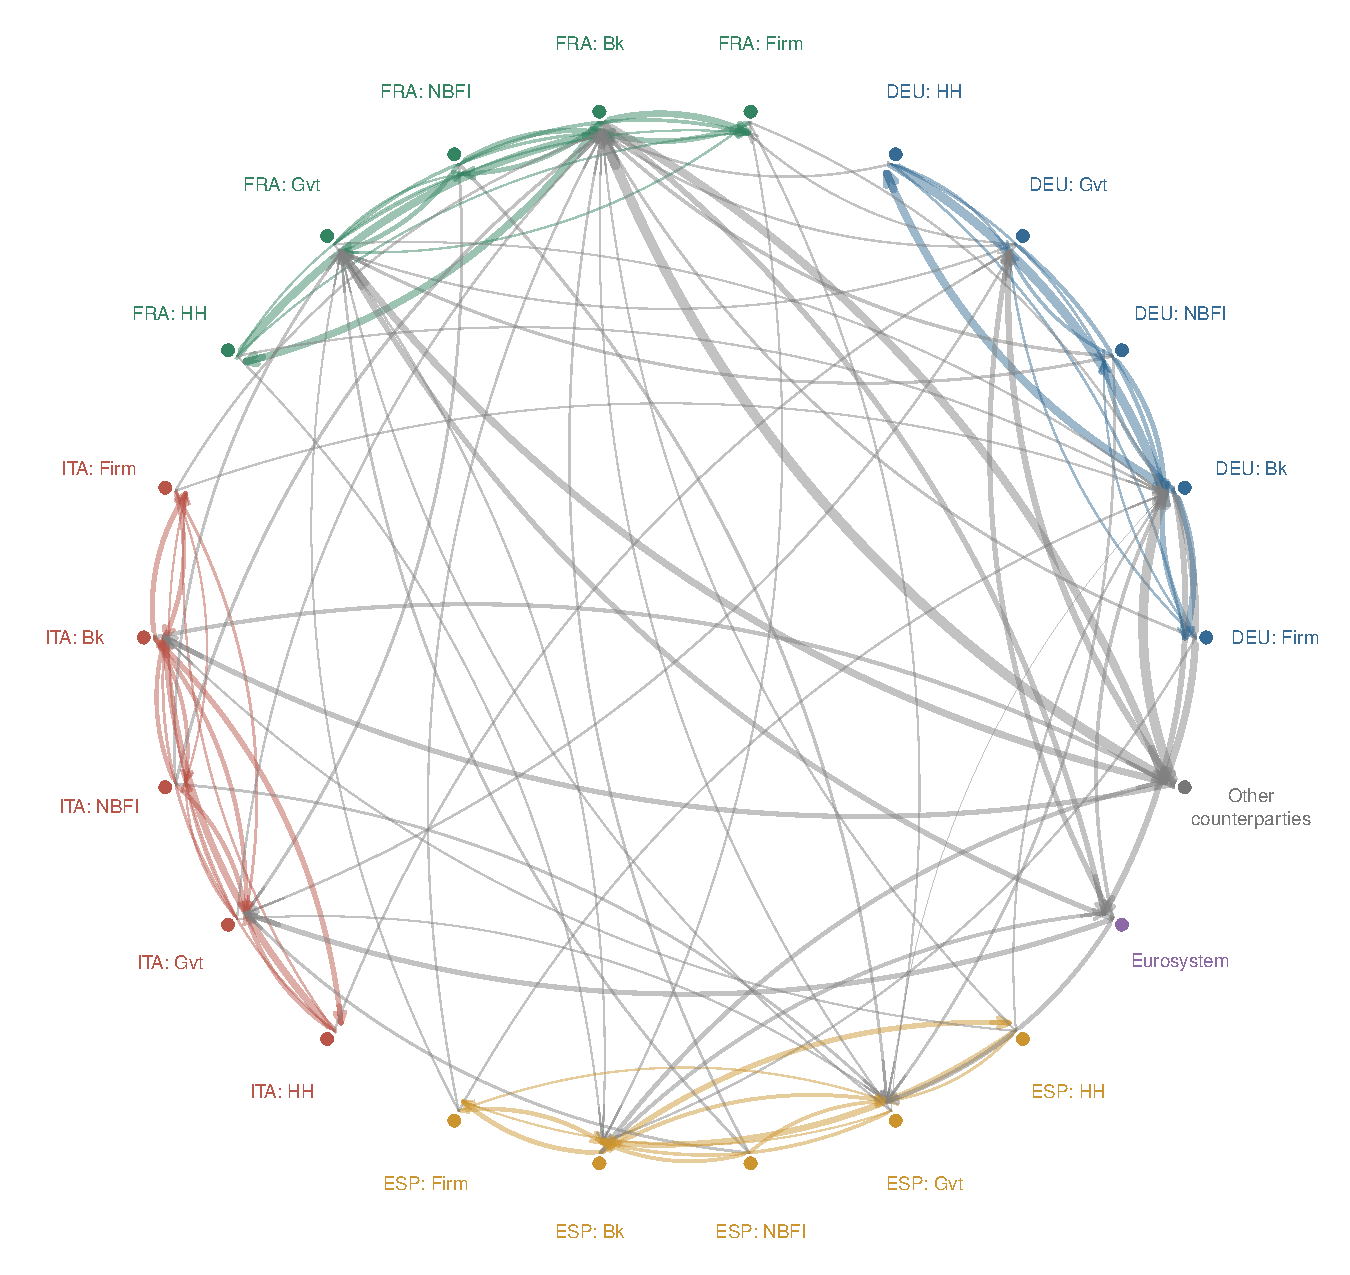
\includegraphics[width=\textwidth]{Figures/figure_network_2024-10-01.pdf}
\end{figure}

\begin{figure}[htbp]
\centering
\floatcaption{Sources represented in the end-2024 residence matrix}{Rows are creditors and columns are debtors. White cells have no positive claim. Cells combining different source layers are marked ``Multiple sources''. Detailed source keys, amounts and reconciliation rules remain in the exposure register.}
\label{fig:active_source_matrix}

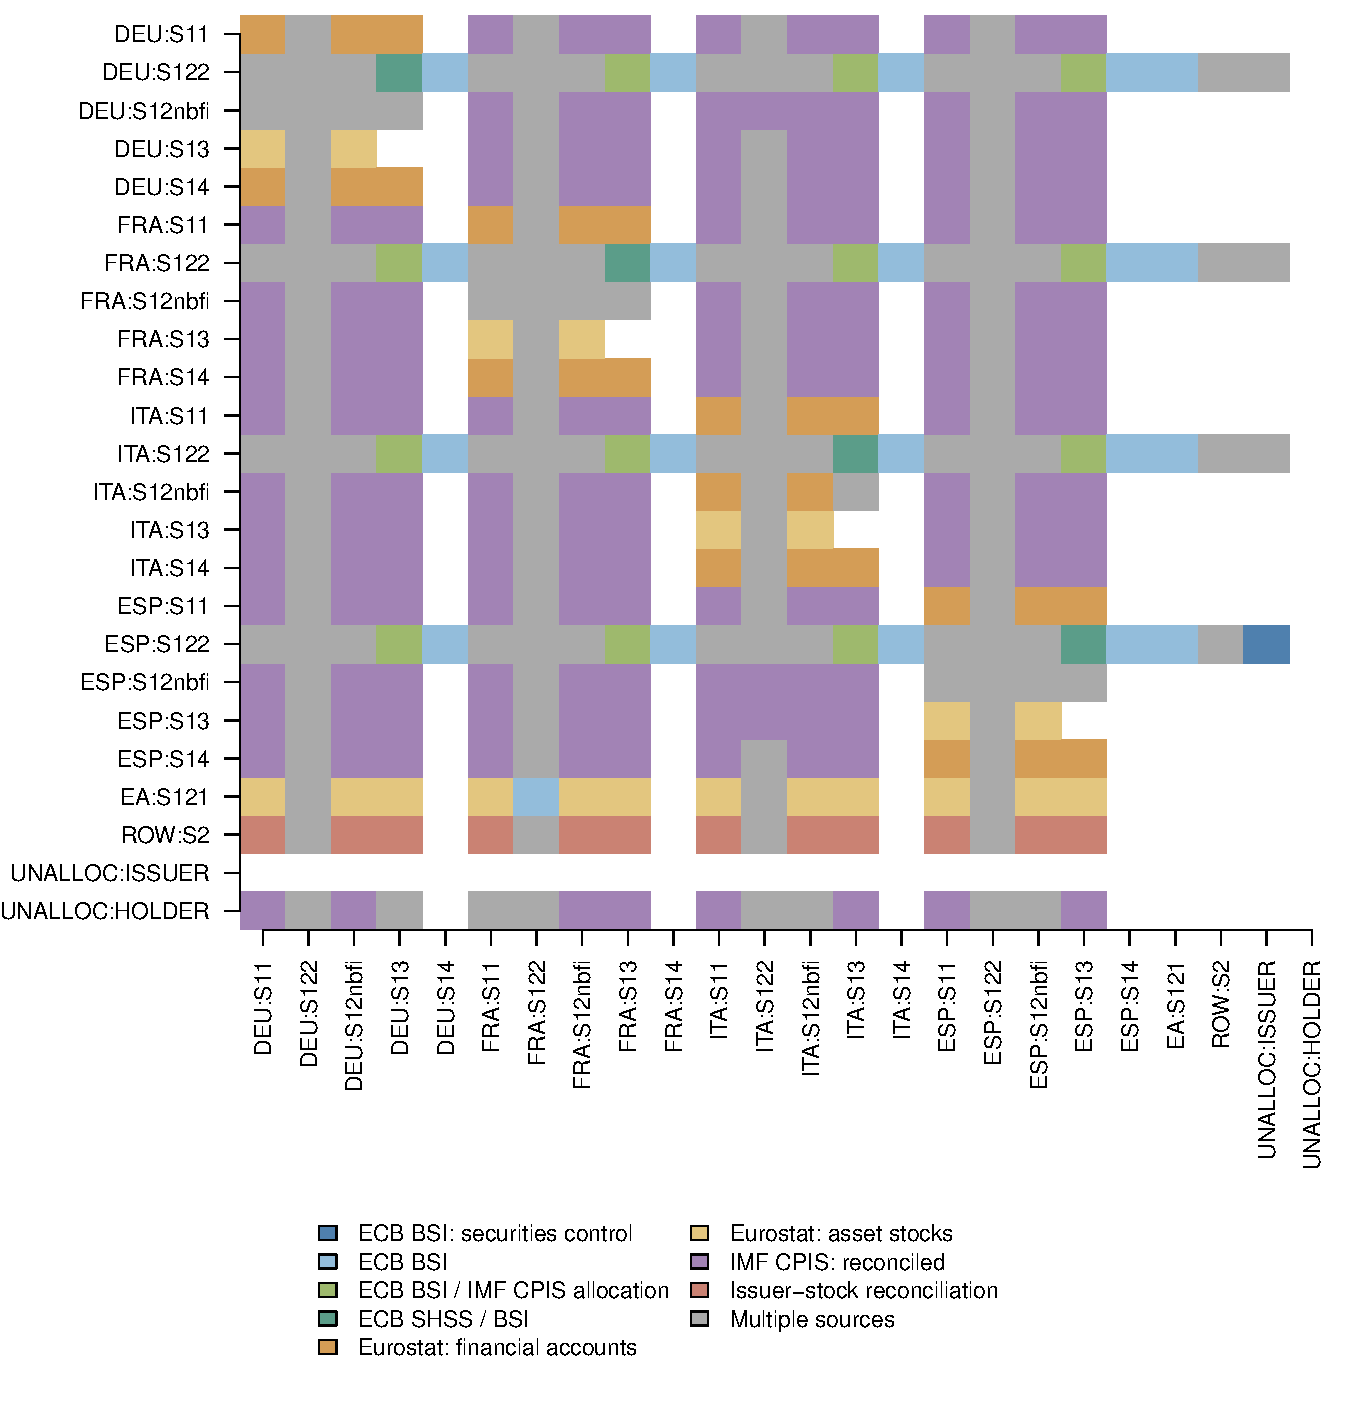
\includegraphics[width=\textwidth]{Figures/active_source_matrix_2024-10-01.pdf}

\end{figure}

The matrix covers selected loans, deposits and debt securities. Other bank assets include government loans, equity holdings, nonfinancial assets and items whose bilateral counterparties are not reconstructed. Coverage and valuation adjustments reconcile these positions to reported balance sheets. Net positions remaining after identified related-office claims are removed are also retained in the reconciliation. These items supply reference repayment resources; they are not independently measured productive wealth.

Write $B_{ij}=x_{ij}$ for banks $i,j$, and $N_{ig}=x_{i,G_g}$ for bank $i$'s holdings of country $g$'s sovereign bonds. Let $D_i^*$ be adjusted statistical liabilities, and let $O_i$ collect net group funding, central-bank funding and remaining or unclassified outside funding settled separately from the common pool. Set
\[
 D_i=D_i^*-O_i,\qquad
 b_i=D_i+E_i-\sum_jB_{ij}-\sum_gN_{ig},
\]
The reference resources therefore satisfy
\[
 b_i+\sum_jB_{ij}+\sum_gN_{ig}=D_i+E_i.
\]
The common pool contains deposits and issued securities. Fixed outside settlements reduce both debt and resources. Provisions against assets are deducted from statistical capital and gross assets together, leaving accounting equity $E_i$. The reference amount $b_i$ includes performing nonbank receipts, outside assets, government loans and coverage or valuation adjustments, net of fixed settlements.

This convention preserves equity but does not assert that the public data identify a single legal recovery class. Remaining liabilities include derivatives and settlement positions, with incomplete public information on close-out rank. The Online Appendix reports the adjustments and statistical-liability benchmarks separately.

\subsection{Prudential headroom and full accounting equity}

For each significant institution, we compute the smaller loss capacity above its published overall risk-weighted capital stack and its leverage requirement. Writing CET1 for Common Equity Tier 1 capital, the country median headroom/CET1 ratio is transferred to resident accounting equity using the same country's public supervisory CET1/equity bridge. Table~\ref{tab:ocr-headroom} reports the resulting headroom and the alternative capacity above a 4.5\% CET1 floor. Consolidated significant institutions and resident offices have different perimeters; these are labelled country proxies, not measured resident regulatory capital.

\begin{table}[htbp]
\centering
\floatcaption{Accounting equity and prudential headroom (EUR billions)}{Equity and clearing debt follow the resident bank balance-sheet reconciliation. OCR headroom uses end-2024 public ECB Pillar 3 and supervisory statistics. ISA headroom is the alternative proxy above a 4.5\% CET1 floor. Neither headroom is substituted for accounting equity in the repayment estate.}
\label{tab:ocr-headroom}
\small

\begin{tabular*}{\textwidth}{@{\extracolsep{\fill}}lrrrr@{}}
\toprule
Country & Accounting equity & Clearing debt & OCR headroom & ISA headroom \\
\midrule
DEU & 686.4 & 7453.6 & 196.8 & 395.5 \\
FRA & 657.0 & 7987.6 & 208.3 & 365.1 \\
ITA & 331.2 & 2697.1 & 90.6 & 168.6 \\
ESP & 245.7 & 2415.9 & 61.5 & 124.5 \\
\bottomrule
\end{tabular*}


\end{table}

Losses exceeding headroom satisfy the first condition for a costly credit event under the disorderly-crisis scenario. An OCR breach can restrict distributions without causing legal default. Market stigma, funding pressure and overlapping constraints can nevertheless impede buffer use \citep{ECBBuffer2023,ECBESRB2026}. The scenario assumes no timely recapitalization or relaxation sufficient to prevent distress. All remaining accounting equity stays in the repayment estate; headroom is never substituted for equity. Partial repayment additionally requires a shortfall after the distress cost.

At the normalized contractual return one, the distress cutoff is $T_i=\min\{D_i+E_i-H_i,D_i/\lambda_i^B\}$. The first term imposes headroom exhaustion; the second ensures that creditors receive less than par on the default branch. Equality gives full repayment. With $H_i=E_i$, the trigger is accounting insolvency; with $\lambda_i^B=1$, the rule becomes ordinary capped pro-rata clearing for any $H_i\leq E_i$.

The baseline $\lambda_i^B=.90$ follows the 10\% remaining-asset default cost in the systemic bank-stress model of \citet{Aikman2009}. It represents realization and franchise disruption in addition to initial credit losses. It is a modelling benchmark, not an estimate of contemporary European administrative resolution costs.

\subsection{Sovereign and private-credit losses}

Safe and contractual bank gross returns equal one. Let $\pi_g^G$ be country $g$'s calibrated annual sovereign-default probability. With 50\% recovery of the contractual payment, sovereign repayments are
\[
 R_g^G(s)=\frac{1-.5\delta_g^G(s)}{1-.5\pi_g^G}.
\]
Mean five-year CDS quotes over December 2007--November 2025 are 14.8, 27.9, 102.5 and 83.9 basis points for Germany, France, Italy and Spain. Let $s_g$ denote these spreads in decimal form. We use them as annual contractual yield-spread proxies, setting $\overline r_g^G=1+s_g$. The expected-payoff normalization $(1-.5\pi_g^G)\overline r_g^G=1$ then gives $\pi_g^G=s_g/[.5(1+s_g)]$, approximately 0.30\%, 0.56\%, 2.03\% and 1.66\%. This is a one-period pricing convention; CDS premium schedules and maturity are not priced separately. These are market-price-based inputs, not historical default frequencies. Marginal risk inputs affect the sovereign payoff normalization; the state comparisons condition on that payoff grid.

The private-credit shock follows the borrower's country. Let $i$ index the creditor's national bank block and $g$ the borrower's country, each among Germany, France, Italy and Spain. The $4\times4$ matrices $\mathbf{F}$ and $\mathbf{Q}$ record bank loans to nonfinancial firms and households, respectively: $F_{ig}$ is the amount lent by banks in country $i$ to firms in country $g$, and $Q_{ig}$ is the corresponding amount lent to households. These loan stocks are extracted from the exposure register; they exclude securities included in the broader sector exposures.

If sovereign $g$ defaults, the scenario imposes an additional loss on those private loans of
\[
 \mathcal L_{ig}=.018F_{ig}+.017Q_{ig}.
\]
For example, a French sovereign default generates private-credit losses for German banks on their loans to French firms and households, even if Germany's sovereign does not default. Summing across borrower countries gives bank $i$'s additional private-credit loss, $\sum_g\mathcal L_{ig}\delta_g^G(s)$, where $\delta_g^G(s)$ equals one if sovereign $g$ defaults in state $s$ and zero otherwise. Its resources before interbank receipts are therefore
\[
 a_i(s)=b_i+\sum_gN_{ig}R_g^G(s)-\sum_g\mathcal L_{ig}\delta_g^G(s).
\]
The sovereign-bond receipts in the second term and the private-loan losses in the third term are distinct channels. The private loss rates, 1.8\% for firm loans and 1.7\% for household loans, are pooled adverse-minus-baseline impairment proxies from the ECB's 2025 bank stress test, Chart 3.8 \citep{ECBStress2025}. Applying them in borrower-country sovereign-default states is a scenario assumption, not an estimated causal relationship. They capitalize a three-year episode once at settlement. Government loans, private securities and outside-sample private loans receive no additional impairment. Opening equity is already net of provisions, so the provision stock is not deducted again. Credit supply and private borrowing remain fixed.

\subsection{NBFI repayment and gross domestic bank claims}

NBFIs have pooled public financial-account buffers and no additional default cost. Financial assets less non-equity liabilities exceed the complete selected bank, NBFI and sovereign claims by approximately EUR~3,500 billion in Germany, 1,329 billion in France, 228 billion in Italy and 377 billion in Spain. With national pooling and other net resources fixed, even zero receipts on these claims leave ordinary debt covered. This establishes par repayment in every equilibrium. An independent eight-node enumeration verifies selected results. Halving NBFI buffer availability also leaves all reported bank equilibrium vectors unchanged.

Identified related-office loans are removed with matched balance-sheet adjustments. The remaining domestic bank claims are retained in $B_{ii}$ as gross obligations among distinct institutions sharing the national repayment rate. The Online Appendix gives a symmetric disaggregation into institutions without own claims that reproduces the block map exactly. It does not rule out asymmetric institutional outcomes. Netting these claims and equal liabilities changes the clearing representation and the estate exposed to costs; this diagnostic removes baseline multiplicity.

\subsection{Weights and comparison with ISA}

Sovereign defaults are independent for the limited set of averages across states reported in the paper; Appendix~\ref{app:ocr_robustness}, Table~\ref{tab:sovereign-dependence}, reports a dependence sensitivity for recovery-backstop averages. In a state with several banking equilibria, the greatest repayment vector receives weight $1-\rho$ and the remaining roots share $\rho$ equally, with $\rho=.20$. A unique root receives weight one. The debt-weighted expected ordinary bank repayment shortfall is approximately 3.0 basis points. State-specific clearing and the maximum capacity over all states do not use these selection weights or the independence convention.

The ECB's Interconnected System-wide stress test Analytics (ISA) application combines granular supervisory and commercial data with liquidity and asset-price feedback \citep{GrassiEtAl2025}. Our public resident-sector network isolates repayment feedback and guarantee capacity. ISA's 4.5\% CET1 default threshold motivates our alternative headroom specification in Appendix~\ref{app:ocr_robustness}, Table~\ref{tab:ocr-robustness} (the row labelled ``ISA headroom''); the baseline uses public OCR/leverage headroom as a conditional distress trigger. The private-credit proxies come from the separate bank stress-test report, not ISA's contagion results. The Online Appendix compares their coverage and thresholds.


\section{An optional household completion}\label{app:household-completion}\label{app:calibration_implementation}

The clearing analysis takes exposures and reference repayment resources as given. This appendix describes a household-saving model that can interpret those positions and their consumption incidence. It is not used to determine exposures, calibrate bank resources or solve any of the reported policy experiments.

\subsection{Complete accounts and household saving}\label{sec:model_households}

Consider complete date-1 accounts. Node $i$ has initial resources $e_i$, absorption $C_i$, lending $X_i=\sum_jx_{ij}$ and borrowing $D_i=\sum_jx_{ji}$. Set $\alpha_{ij}=x_{ij}/X_i$ when $X_i>0$, and use any nonnegative portfolio-share row summing to one when $X_i=0$. Bold symbols denote vectors, and $\boldsymbol\alpha=(\alpha_{ij})$ is the portfolio-share matrix. The accounts satisfy
\[
 e_i+D_i=C_i+X_i,\qquad
 \mathbf D=\boldsymbol\alpha^\top\mathbf X,
 \qquad \mathbf e=\mathbf C+\mathbf X-\mathbf D.
\]
Set $C_{H_c}=c_{1,c}$ and $C_i=0$ for other nodes. These identities concern complete accounts; the selected empirical network instead uses the bank reconciliation to supply omitted resources, clearing debt and accounting equity. Initial resources $e_i$ are distinct from bank accounting equity.

Let $Y_{2,c}(s)$ be nonportfolio resources, $P_{H_c}(s)$ the household debt payment, $\beta>0$ the discount factor, and $u_c^0,u_c^1,u_c^2$ utility coefficients, with $u_c^2>0$. Let $r$ and $r^R$ denote the reference private and safe gross returns, both normalized to one in the quantitative exercise. These resources and debt payments are given. The reference debt payment is $rD_{H_c}$; scenario payments may reflect the specified impairment of bank-held household loans. On household-held claims, $R_j$ is the realized government or bank repayment when the debtor is a sovereign or bank, $r$ for the other domestic sectors under the baseline par-repayment result, and $r^R$ for the Eurosystem and Other counterparties. Instrument-specific scenario payoffs can be incorporated without changing the saving argument.

Household $H_c$ takes borrowing, portfolio shares and the distribution of claim repayments as given. It chooses $c_{1,c}\geq0$ and $X_{H_c}\geq0$ to maximize
\[
 u_c(c_{1,c})+\beta\mathbb E[c_{2,c}],\qquad
 u_c(c)=u_c^0+u_c^1c-\frac{u_c^2}{2}c^2,
 \quad u_c^2>0,\quad\beta>0,
\]
subject to
\[
 e_{H_c}+D_{H_c}=c_{1,c}+X_{H_c},\qquad
 c_{2,c}(s)=Y_{2,c}(s)+X_{H_c}\sum_j\alpha_{H_c,j}R_j(s)-P_{H_c}(s).
\]

The objective is strictly concave in $c_{1,c}$, with second derivative $-u_c^2<0$. At an interior solution, $u_c^1-u_c^2c_{1,c}=\beta\mathbb E[\sum_j\alpha_{H_c,j}R_j]$, giving
\[
 X_{H_c}=e_{H_c}+D_{H_c}-\frac{u_c^1}{u_c^2}
       +\frac{\beta}{u_c^2}\mathbb E\!\left[\sum_j\alpha_{H_c,j}R_j\right].
\]
This condition is not imposed in calibration or clearing: exposures are observed or reconstructed inputs. The completion does not model firms' portfolio choices or credit-supply responses.

\subsection{Consumption and utility differences}

Fix a sovereign state and compare two banking equilibria with identical portfolios, debt payments and nonportfolio resources. Their date-2 consumption difference equals their receipt difference. With NBFIs repaying in full, only bank payments vary, yielding the expression in Section~\ref{subsec:household-macro-implications}.

With date-1 consumption fixed, full pass-through of receipts to date-2 consumption and no other transfers or financing costs, the conditional utility gain from selecting the preferred equilibrium is $\beta\Delta c_{2,c}^e(s)$. Deposit protection and its financing can change that incidence. These assumptions do not turn gross receipt differences into estimates of realized consumption or welfare gains; neither consumption levels nor preference parameters enter their calculation.


\section{Robustness of the crisis specification}\label{app:ocr_robustness}

Table~\ref{tab:ocr-robustness} varies public headroom definitions and selected crisis assumptions while preserving the residence matrix and full bank accounting equity. All cases use $\lambda=.90$ except the minimum-requirement row. In 75 joint local combinations, OCR headroom varies from 90\% to 110\% of its reference value, $\lambda$ from .89 to .91, and both private-loss rates by $\pm.1$ percentage point. Multiplicity persists in 3--10 states throughout; defaults under full interbank repayment occur in twelve states and the no-sovereign-default state stays unique. These are scenario sensitivities, not confidence intervals.

\begin{table}[htbp]
\centering
\floatcaption{Public-threshold and crisis sensitivities}{Default states count sovereign states with at least one bank default under full interbank repayment; bank--state events count individual bank-country/state pairs with such defaults. This diagnostic applies sovereign and private-credit losses while assuming full payment of every interbank claim. All counts concern sixteen sovereign states. Lower/upper quartiles describe cross-bank headroom ratios; they are not estimated national confidence bounds. NBFI availability of 50\% leaves all bank equilibrium vectors unchanged.}
\label{tab:ocr-robustness}
\small

\begin{tabular*}{\textwidth}{@{\extracolsep{\fill}}lrrr@{}}
\toprule
Specification & Default states & Bank--state events & Multiple states \\
\midrule
ISA headroom, $\lambda=.90$ & 12 & 16 & 0 \\
Half ISA headroom, full equity & 12 & 22 & 3 \\
Public median OCR (baseline) & 12 & 16 & 8 \\
Lower-quartile OCR & 14 & 24 & 8 \\
Upper-quartile OCR & 12 & 16 & 6 \\
Minimum requirements, $\lambda=.875$ & 12 & 16 & 8 \\
Sovereign recovery 55\% & 12 & 16 & 8 \\
Sovereign recovery 45\% & 12 & 16 & 7 \\
NBFI availability 50\% & 12 & 16 & 8 \\
\bottomrule
\end{tabular*}


\end{table}

Admitting 25\%, 50\%, 75\% and 100\% of the capacity between OCR and minimum requirements leaves 8, 6, 4 and 2 multiple states, respectively. With a 5\% default cost, multiplicity disappears. Netting domestic bank claims and equal liabilities also removes multiplicity, showing the role of gross domestic exposures. The online appendix provides their symmetric-institution interpretation.

\paragraph{Average losses and payments under the recovery backstop}
Section~\ref{sec:interbank-recovery-backstop} reports state-by-state equilibrium effects and maximum payments. Figure~\ref{fig:backstop-weighted-averages} additionally summarizes average outcomes. In each sovereign state, the preferred policy equilibrium receives weight $1-\rho$ and the others share $\rho$ equally; a unique equilibrium receives weight one. We consider $\rho\in\{.1,.2,.3\}$. Crisis-conditional averages then weight sovereign states using the independent marginal risk inputs from Section~\ref{subsec:calibration_choices}. Interbank credit loss is the claim-weighted shortfall $\sum_jL_j^{BB}[1-\widehat R_j^e(s;\eta)]/\sum_jL_j^{BB}$. A state-expected payment averages over equilibria within a given sovereign state; its maximum across states can differ from the maximum across individual equilibria reported in the main text.

At half coverage and $\rho=.20$, payments conditional on a sovereign crisis are 0.05\% of aggregate bank debt, and conditional interbank credit losses fall from 44.2 basis points without intervention to 3.1 basis points. Since half coverage gives a unique equilibrium in every sovereign state, its policy outcomes do not depend on $\rho$; the comparison without intervention does. Dependence between sovereign defaults affects these crisis-conditional averages, as examined below.

\begin{figure}[htbp]
\centering
\floatcaption{Recovery-backstop averages under alternative equilibrium-selection weights}{Coverage is evaluated in five-percentage-point steps and $\rho\in\{.1,.2,.3\}$. Panel (a) counts states with multiplicity. Panels (b) and (c) report interbank credit losses and payments conditional on a sovereign crisis under independent defaults. Panel (d) gives the largest within-state expected payment. Payments are percentages of aggregate bank debt; interbank losses are basis points of interbank claims.}
\label{fig:backstop-weighted-averages}

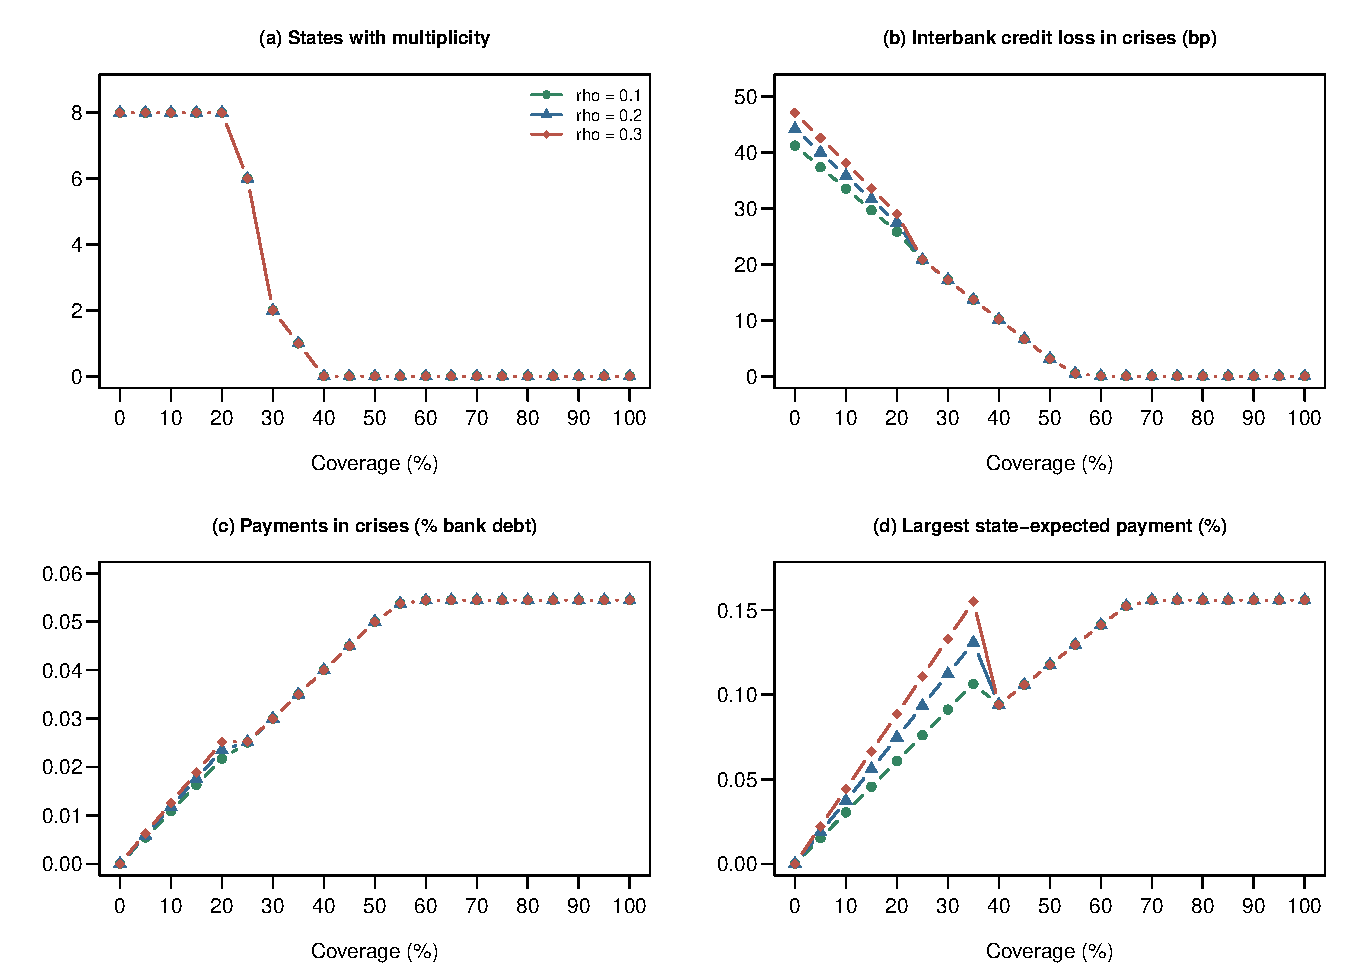
\includegraphics[width=\linewidth]{Figures/interbank_recovery_backstop_averages.pdf}

\end{figure}

\paragraph{Dependence between sovereign defaults}
Independence affects averages across sovereign states, not the equilibrium solutions conditional on a state. Table~\ref{tab:sovereign-dependence} reweights the saved equilibria while keeping each country's marginal default probability, sovereign payments and within-state equilibrium weights ($\rho=.20$) fixed. We mix independence with a shared-shock distribution: for a single uniform random variable $U$, country $g$ defaults when $U<\pi_g^G$. A mixture weight of one is the fully shared-shock case.\footnote{For the 50--50 mixture, imagine tossing a single fair coin for all four countries, before conditioning on a sovereign crisis. On heads, their defaults are independent, with the calibrated probabilities: approximately 0.30\% for Germany, 0.56\% for France, 2.03\% for Italy and 1.66\% for Spain. On tails, draw a single $U$ uniformly between zero and one and compare it with each country's default probability. For example, $U=0.4\%$ implies default in France, Italy and Spain, while $U=1\%$ implies default only in Italy and Spain. Defaults are thus nested under the shared shock: whenever a lower-risk sovereign defaults, all higher-risk sovereigns default too. Each sovereign configuration receives half its probability under independence plus half its probability under the shared shock. Each country's individual default probability is unchanged because it is the same under both mechanisms. The 50\% is the probability of selecting the shared-shock mechanism, rather than a default correlation of 50\%.} This is a dependence stress, not an estimate of sovereign correlations.

\begin{table}[htbp]
\centering
\floatcaption{Sovereign-dependence sensitivity of recovery-backstop averages}{B--B losses and payments are conditional on at least one sovereign default. Losses are basis points of interbank claims; payments are percentages of aggregate clearing debt. The shared-shock weight changes the joint distribution while preserving marginal default probabilities. All state-specific equilibria and all-state commitment capacities remain unchanged.}
\label{tab:sovereign-dependence}
\small

\begin{tabular*}{\textwidth}{@{\extracolsep{\fill}}lrrrr@{}}
\toprule
Dependence & \shortstack{Crisis probability\\(\%)} & \shortstack{B--B loss\\$\eta=0$ (bp)} & \shortstack{B--B loss\\$\eta=.50$ (bp)} & \shortstack{Payment\\$\eta=.50$ (\% debt)} \\
\midrule
Independent & 4.48 & 44.2 & 3.1 & 0.05 \\
50\% shared-shock mixture & 3.26 & 65.5 & 8.1 & 0.07 \\
Fully shared shock & 2.03 & 112.6 & 18.9 & 0.11 \\
\bottomrule
\end{tabular*}

\end{table}

Positive dependence increases the frequency of joint defaults relative to isolated defaults, raising crisis-conditional losses and payments. At half coverage, the conditional payment rises from 0.05\% of bank debt under independence to 0.11\% under the fully shared shock. Conditional interbank losses fall from 112.6 to 18.9 basis points when half coverage is introduced in that stress, compared with a fall from 44.2 to 3.1 under independence. The largest within-state expected payment remains 0.12\% of bank debt, and half coverage still eliminates multiplicity in every sovereign state. Thus the effectiveness result is unchanged, while the probability-weighted magnitudes depend on sovereign dependence.


\section{Implementation of the sovereign-bond purchases}\label{app:purchase-implementation}

Purchases take place before the sovereign state is realized. Banks exchange a specified fraction of their holdings of selected sovereign issuers for an equal reserve claim at the model book value of one. They are not sales of defaulted debt at par. Let $\mathbf{P}=(P_{ig})$ be the purchase matrix, $\mathbf{N}=(N_{ig})$ the bank sovereign-bond matrix defined in Appendix~\ref{app:calibration-details}, and $\mathbf{b}=(b_i)$ the reference-resource vector. With $\mathbf1$ the vector of ones and primes denoting post-purchase positions, the bank resource equation changes through
\[
 \mathbf{N}'=\mathbf{N}-\mathbf{P},\qquad \mathbf{b}'=\mathbf{b}+\mathbf{P}\mathbf1.
\]
The reporting matrix deducts $P_{ig}$ from bank $i$'s claim on government $g$, adds $\sum_iP_{ig}$ to the Eurosystem's claim on that government, and adds $\sum_gP_{ig}$ to bank $i$'s reserve claim. Eurosystem assets and liabilities both expand by $\sum_{ig}P_{ig}$. Government debt columns, bank asset totals, clearing debts, accounting equity and headroom remain unchanged. Capital requirements and private-credit impairments are not recomputed.

For fixed bank repayments, the aggregate resource gain equals the Eurosystem's additional net cash shortfall,
\[
 \sum_i\Delta A_i(s)=\sum_{ig}P_{ig}[1-R_g^G(s)].
\]
This quantity can be negative in survival states because sovereign receipts exceed the reserve payment under the existing payoff normalization. Its expectation under the model's pricing probabilities is zero by construction, not an estimate of economic or fiscal cost. Maximum state shortfalls are approximately EUR~75 billion for half of French holdings and EUR~290 billion for half of all sample-issuer holdings. National central-bank loss sharing and fiscal responses are outside the model. The Online Appendix explains this limitation and the corresponding public purchase arrangements.

All sixteen bank default regimes are re-enumerated in each of the sixteen sovereign states after each exchange. The NBFI buffer bound continues to support full repayment. Independent eight-node enumeration confirms the results in all states for purchases of half of all sample-issuer holdings, half of French holdings and three quarters of Italian and Spanish holdings. A zero purchase reproduces every baseline equilibrium. Checks also verify balance-sheet identities, sovereign debt totals, unchanged equity and headroom, and equality of direct bank resource gains and Eurosystem cash exposure. The proportional-floor calculation is repeated on each counterfactual network, including the critical-capacity endpoint check. No optimization over purchase size or composition is claimed.



\bibliographystyle{elsarticle-harv}
\bibliography{Biblio}

\end{document}
